\documentclass[12pt, a4paper,twoside,openany]{report} %openany= standard openright=für druck
\usepackage[utf8]{inputenc} %Standard!
\usepackage[english,ngerman]{babel} %für deutsch
% Bibliotheken und Pfade
\usepackage{csquotes} %damit zitierung konsisntent mit sprache ist
\usepackage{xcolor} %Farben
\usepackage{graphicx, wrapfig} %Bilder
\usepackage{subfig} %Bilder erweiterung
\usepackage{setspace, geometry} %margins
\usepackage{mathptmx} %Wir benutzen hier eine Mathebibiliothen um Times new Roman zu verwenden
\usepackage[T1]{fontenc} %Standard!
\usepackage{setspace} %zeilenabstände
\usepackage{float}
\usepackage{listings} %code darstellung
\usepackage{dirtytalk} %zitieren
\usepackage{pdfpages} %pdf hinzufügen
\usepackage[backend=biber, style=ieee, sorting=none]{biblatex} %references
\usepackage{titlesec} %zum entfernen der "Kapitel N" header
\usepackage{abstract} %zusammenfassung / Abstract
\usepackage{listings} %zum code darstellen
\usepackage{courier} %textstyle

% pdf hyperref
\usepackage[
    bookmarks=true,
    bookmarksopen=true,
    bookmarksnumbered=true,
    bookmarksopenlevel=1,
    pdfpagelabels=true,
    colorlinks=true,
    linkcolor={blue!80!black},
    urlcolor={blue!80!black},
    anchorcolor=black,
    citecolor={blue!80!black},
    filecolor={blue!80!black},
    menucolor=black,
    plainpages=false,
    hypertexnames=true,
    linktocpage=true,
]{hyperref}

%code darstellung
\lstset{basicstyle=\footnotesize\ttfamily,breaklines=true}
\lstset{framextopmargin=10pt,framexbottommargin=10pt,frame=lines,numbers=left,}

%Abstract seite
\renewenvironment{abstract}{
  \vspace*{\fill}
  \begin{center}%
    \bfseries\abstractname
  \end{center}}%
  {\vfill}

%wir wollen formatieren{was genau?}[optionaler argument: im block satz.]{kapitel nummerierung und font}{der kapitelname mit angehängtem punkt .}{abstand zwischen nummer und name}{größe titel}
\titleformat{\chapter}[block]{\normalfont\Large\bfseries}{\thechapter.}{1em}{\Large}

\titlespacing*{\chapter}{0pt}{40pt}{30pt} % this alters "before" spacing (the second length argument) to 0
%\titlespacing*{\chapter}{0pt}{50pt}{40pt} % default

\graphicspath{ {images/} }

\geometry{paper=a4paper,left=2.5cm,top=3.0cm,bindingoffset=0.8cm}
\onehalfspacing
\setlength{\belowcaptionskip}{-10pt}

\addbibresource{refs.bib}

% Baue die Titel Struktur + Inhalt
\title{
{\vspace{-20mm}}
\begin{figure}[H]
    \centering
    
\includegraphics[width=0.6\linewidth]{images/Ohm.png}%
\end{figure}

{\huge Wave-Function-Collapse}\\
{\large Funktionsweise und Anwendungsfälle}\\
{\vspace{10mm}}
{\large Bachelorarbeit}\\
{\large Betreuer: Prof. Dr. Matthias Hopf}\\
{\vspace{10mm}}
{\large Studiengang: Bachelor Media Engineering}\\
{\large Fakultät: Elektrotechnik Feinwerktechnik Informationstechnik}\\

% Setze Author und Datum
\author{
    Davoud Tavakol \\ Matrikelnummer: 3540912
}
\date{{\vspace*{\fill}}  \raggedright{Sommersemseter 2023 \\ Abgabedatum: 20. Juli 2023}}
}

% Start Dokument
\begin{document}

% Erstelle den Titel (Dieser Befehlt setzt dann auch den Author und das Datum!)
\maketitle

%Eidesstaatliche Erklärung
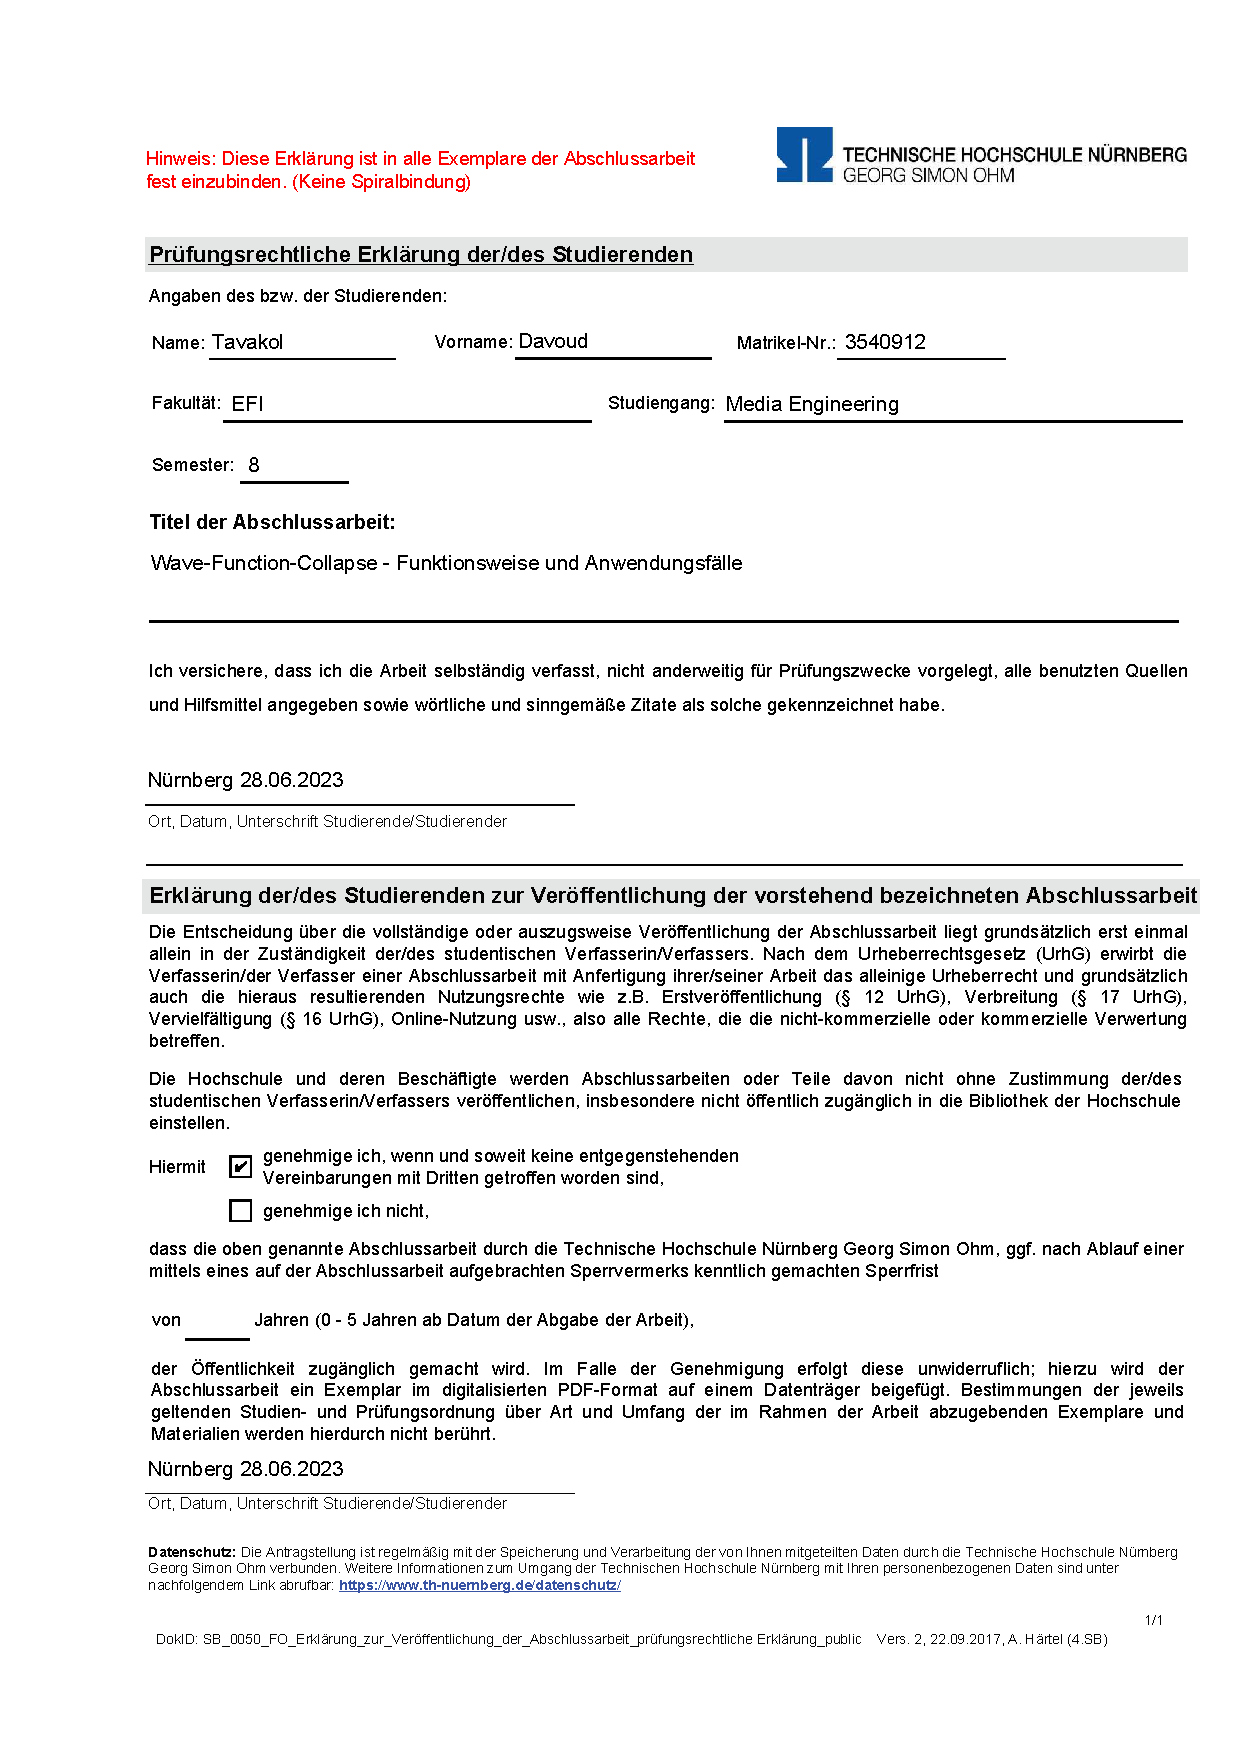
\includepdf[pages=-]{Davoud_Tavakol_Pruefungsrechtliche_Erklaerung.pdf}

\begin{abstract}
In dieser Bachelorarbeit wird auf die Funktionsweise des Wave-Function-Collapse {(WFC)} Algorithmus von Maxim Gumin eingegangen und wie dieser für Textursynthesen sowie zur Erstellung
von prozedural generierten Content verwendet werden kann.
Dazu wird zuerst auf gängige Textursynthese Algorithmen eingegangen und inwiefern sich WFC von diesen Unterscheidet.
Später wird die Model Synthese von Paul Merrell herangezogen um Ähnlichkeiten zwischen den beiden Algorithmen aufzuzeigen und zu verglichen.
Es wird klar das beide Algorithmen sich in ihrer Methodik sogenannte Constraint-Satisfaction-Probleme {(CSP)} zu lösen als identisch erweisen.
Danach werden die Unterschiede der jeweiligen Implementierungen der Algorithmen aufgezeigt, wie z.B. die Blockweise Generierung der Model Synthese und das Overlapping Model von Gumin.
Zum Schluss wird das Overlapping Modell detailliert dargestellt und darauf eingegangen, weshalb diese Implementation zu Bekanntheit gelangt ist und welche Anwendungsfälle mit WFC
generell möglich sind.
\end{abstract}

\selectlanguage{english}
\begin{abstract}
This bachelor thesis describes the Wave-Function-Collapse {(WFC)} algorithm by Maxim Gumin and how it can be used for texture synthesis and the creation of procedurally generated content.
Firstly, common texture synthesis algorithms and how WFC differs from them are discussed.
Later, the model synthesis of Paul Merrell is used to show similarities between the two algorithms and compare them.
It becomes clear that both algorithms are identical in their methodology to solve so-called constraint satisfaction problems {(CSP)}.
Afterwards, the different implementations of the respective algorithms are pointed out, such as the modifying in blocks generation of the model synthesis and the overlapping model of Gumin.
Finally, the Overlapping Model is explained in detail and why this implementation has gained so much attention lately and which use cases are generally possible with WFC.
\end{abstract}

% Automatisches Inhaltsverzeichniss
\selectlanguage{ngerman}
\tableofcontents

\chapter{Einleitung}

Die automatische Generierung von Inhalten wie Texten, Bildern oder Modellen ist heutzutage Standard in vielen Bereichen der Industrie.
Um solche Inhalte mit vordefinierten Parametern zu erstellen, werden oft zwei Methoden zur Generierung verwendend.
AI's {(Künstliche Intelligenzen)} wie DALL-E2, Midjourney und Algorithmen wie die Patch Synthese.
Vorteile dieser Werkzeuge ist es, dass sie in kurzer Zeit qualitativ hochwertige Resultate Generieren können und auch, wie oben erwähnt,
vordefinierte Parameter als Input erhalten können, um die Resultate für ihren Gebrauch anzupassen.
In dieser Bachelorarbeit wird auf den von Maxim Gumin erstellten Wave-Function-Collapse Algorithmus, dessen Herkunft, Funktionsweise und Anwendungsfälle eingegangen.
Zuerst werden gängige nicht interaktive Textursynthesen wie die Pixel basierte Textursynthese, Pyramid basierte Textursynthese und der Patch basierte Textursynthese erläutert
und wie Wave-Function-Collape sowie andere Textursynthesen davon inspiriert wurden.
Daraufhin wird das Konzept zum Lösen von Constraint-Satisfaction-Problemen {(CSP)} und die Funktionsweise vom WFC Algorithmus, solche Probleme zu lösen, dargestellt.
Anhand eines Beispiels wird im Detail die Funktionsweise zum Lösen solcher CSP's aufgezeigt.
Wave-Function-Collapse als Algorithmus für Procedural-Content-Generation {(PCG)} wird mit der Model Synthese von Paul Merrell verglichen und deren Unterschiede genauer betrachtet.
Es wird deutlich, dass der Wave-Function-Collapse Algorithmus sowie die Model Synthese beide sowohl in Ihrer Verwendung von Pixelganuer / diskreten Synthese sowie im Lösen von
CSP ähnliche Methoden verwenden und beide sich dadurch als PCG's verwenden lassen.
Dadurch kann der Output dieser Algorithmen interaktiv als Content verwendet werden wie beispielsweise für Videospiele etc.

\chapter{Textursynthesen im Vergleich}

Es gibt viele Möglichkeiten Textursynthese mit Algorithmen zu erzielen.
Die meisten dieser Methoden basieren auf demselben Grundprinzip, aus kleineren Input-Images größere oder gleich große Output-Images zu generieren.
Nach D.Gomathi und Rajvi Shah \cite[S.1]{GomathiShah2009}, kann die Textursynthese wie folgt definiert werden.
\newline
Ziel einer Textursynthese ist es aus einer Texturprobe eine neue Textur zu generieren, die, \say{wenn sie von einem menschlichen Beobachter wahrgenommen wird,
durch denselben zugrundeliegenden Prozess erzeugt wird.}
Das Ergebnis muss der Texturprobe ähnlich sein aber dennoch in der Wahrnehmung genügend Variation enthalten.
Eine solche Synthese ist nicht möglich, wenn man die Eingabetextur einfach mehrfach kachelt.
Dadurch erhält man keine \say{sauberen} Übergänge, und die einzelnen Blöcke sind klar erkennbar {(siehe Abbildung 2.1)}.

\begin{figure}[H]
    \centering
    \subfloat[][]{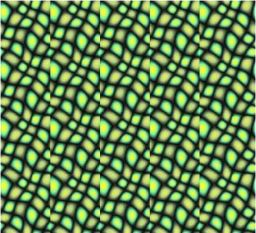
\includegraphics[width=0.4\linewidth]{images/texture-blocky.JPG}}%
    \qquad
    \subfloat[][]{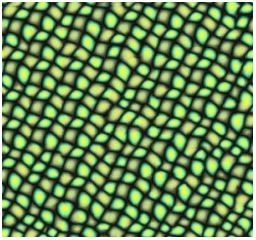
\includegraphics[width=0.4\linewidth]{images/texture-correct.JPG}}%
    \caption{(a) Blockartige Textur, (b) Textursynthese}%
\end{figure}

\paragraph{Dadurch ergeben sich folgende Metriken, die erfüllt werden müssen.}

\begin{itemize}
    \item Bei gegebener Texturprobe, generiere eine neue Textur, die der Probe gleicht.
    \item Die neue Textur kann eine beliebige Größe haben, die vom Benutzer festgelegt wird.
    \item Es sollen keine sichtbaren Übergänge, Artefakte oder fehlerhafte Kanten sichtbar sein.
    \item Dasselbe Muster soll nicht mehrfach in der neuen Textur vorkommen. \cite[S.2]{GomathiShah2009}
\end{itemize}

Im Folgenden soll auf drei in ihrem Prinzip und ihrer Wirkungsweise unterschiedliche Textursyntheseverfahren eingegangen werden,
um damit verschiedene Ansätze von Synthesen aufzuzeigen.
Da eine vertiefte Diskussion für diese Arbeit nicht relevant ist, werden hierbei lediglich die groben Prinzipien / Hintergrundinformationen geklärt.

\section{Pixel basierte Textursynthese}

Bei dieser Methode werden neue Texturen Pixel für Pixel generiert.
Jeder neue Pixelwert wird von seinen lokalen Nachbarn festgelegt.
Diese Verfahren verwenden meistens Markow-Netzwerke \textit{(Markov Random Field)},
\footnote[1]{Auf Markow-Netzwerke und Markow-Ketten wird am Ende dieses Abschnitts genauer eingegangen.}
die relativ gute Resultate liefern mit wenig Rechenlast.
Markov Random Fields Methoden beurteilen jeden Pixel nach einer kleinen Menge von Nachbarn.
Voraussetzung hierfür ist, dass das Input-Image stationär und lokal ist.
Ein Image wird als stationär bezeichnet, wenn unter korrekter Fenstergröße,
jeder betrachtete Bereich ähnlich zueinander aussieht.
Lokal ist ein Image dann, wenn jeder Pixel allein von seinen Nachbarn bestimmt werden kann \cite{GomathiShah2009}.

\begin{figure}[H]
    \centering
    \subfloat[][]{\frame{\includegraphics[width=0.45\linewidth]{images/Textur-nicht-stationärlokal.JPG}}}%
    \qquad
    \subfloat[][]{\frame{\includegraphics[width=0.45\linewidth]{images/Textur-stationärlokal.JPG}}}%
    \caption{(a) Nicht stationär und lokal, (b) stationär und lokal.}%
\end{figure}

Unterschiedliche Bereiche einer Textur sehen sich immer ähnlich {(siehe Abbildung 2.2 (b))}.
Dies ist nicht der Fall für normale Images wie wir bei Abbildung 2.2 {(a)} erkennen können.
Zudem ist es möglich jeden Pixel in {(b)} allein durch seine benachbarten Pixel zu bestimmen.
Diese Attribute bezeichnet man als Stationär und Lokal \cite{GomathiShah2009}.
Im Folgenden ist die Funktionsweise eines Algorithmus basierend auf Markov Random Fields nach Efros und T. Leung dargestellt: \cite{Efros99}

\begin{figure}[H]
    \centering
    \subfloat[][]{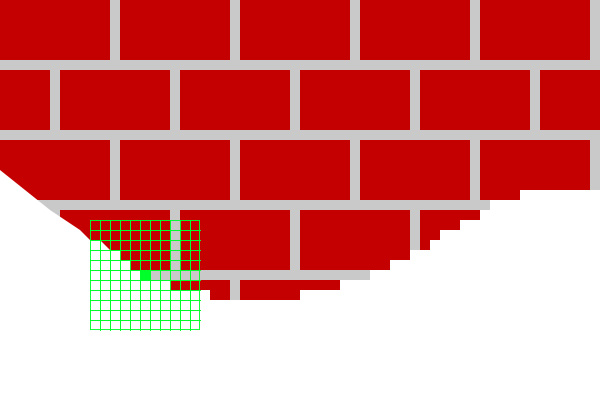
\includegraphics[width=0.45\linewidth]{images/synthezising-pixel.JPG}}%
    \qquad
    \subfloat[][]{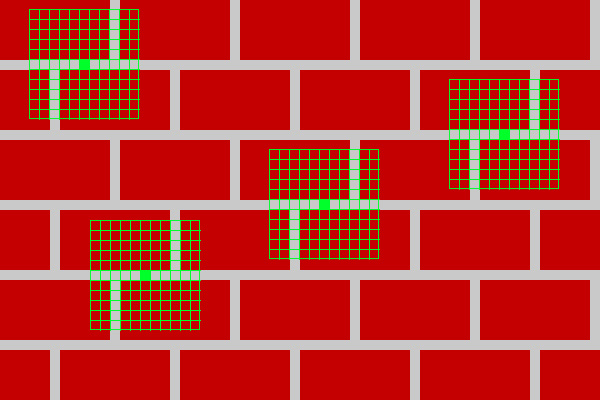
\includegraphics[width=0.45\linewidth]{images/Wall-sample.JPG}}%
    \caption{(a) Pixelsynthese, (b) Sampling des Input-Images.}%
\end{figure}


\begin{itemize}
    \item Zuerst wird vom Input-Image eine Teiltextur einer bestimmten Größe {(z.B. $5\times 5$ Pixel Fenster)} ausgewählt. Von diesem Feld aus werden Spiralförmig neue Pixel generiert.
    \item Für jeden Pixel der betrachtet wird, wird ein Fenster einer selbst bestimmten Größe zentral über das Pixel gelegt. 
    Die Größe des Fensters muss nach Größe der einzelnen Elemente der Textur gewählt werden  {(siehe Abbildung 2.3 (a))}.
    \item Mit dieser Gruppe von Pixel {(der Zentrale Pixel und alle seiner Nachbarn im Fenster)} werden nun alle im Input-Image ähnlichen $N$ Kandidaten gesucht {(siehe Abbildung 2.3 (b))}.
    \item Danach wird zufällig aus einer dieser möglichen Kandidaten einer ausgewählt und der betrachtete Pixel im Output wird aus diesem Kandidaten kopiert.
    \item Dieser Prozess wiederholt sich so lange, bis alle nicht bekannten Pixel generiert wurden \cite[S.4]{GomathiShah2009}.
\end{itemize}

\subsubsection{Markow-Netzwerk und Markov-Kette}

Wie bereits erwähnt basieren einige Textursynthesen auf sogenannten Markow-Netwerke oder Markov-Ketten \textit{(Markov Chain)}.
In diesem Abschnitt wird kurz erklärt, um was es sich genau bei diesen beiden Begriffen handelt.\par
Ein Markow-Netwerk kann als Generalisierung einer Markow-Kette im 3D-Raum angesehen werden.
Eine Markow-Kette dient dazu Wahrscheinlichkeiten zukünftiger Ereignisse anzugeben.
Sie basiert auf der Theorie, dass bereits begrenzte Informationen über den vergangenen Zustand eines Systems ausreichen,
um Prognosen für die zukünftige Entwicklung des Systems zu erstellen.
Die Markow-Kette, oder auch Markow-Kette erster Ordnung, beschreibt konkret:
\say{Der zukünftige Zustand des Prozesses ist nur durch den aktuellen Zustand bedingt und wird nicht durch vergangene Zustände beeinflusst.} \cite{wiki:Markow-Kette}

\begin{figure}[H]
    \centering
    \subfloat[][]{\frame{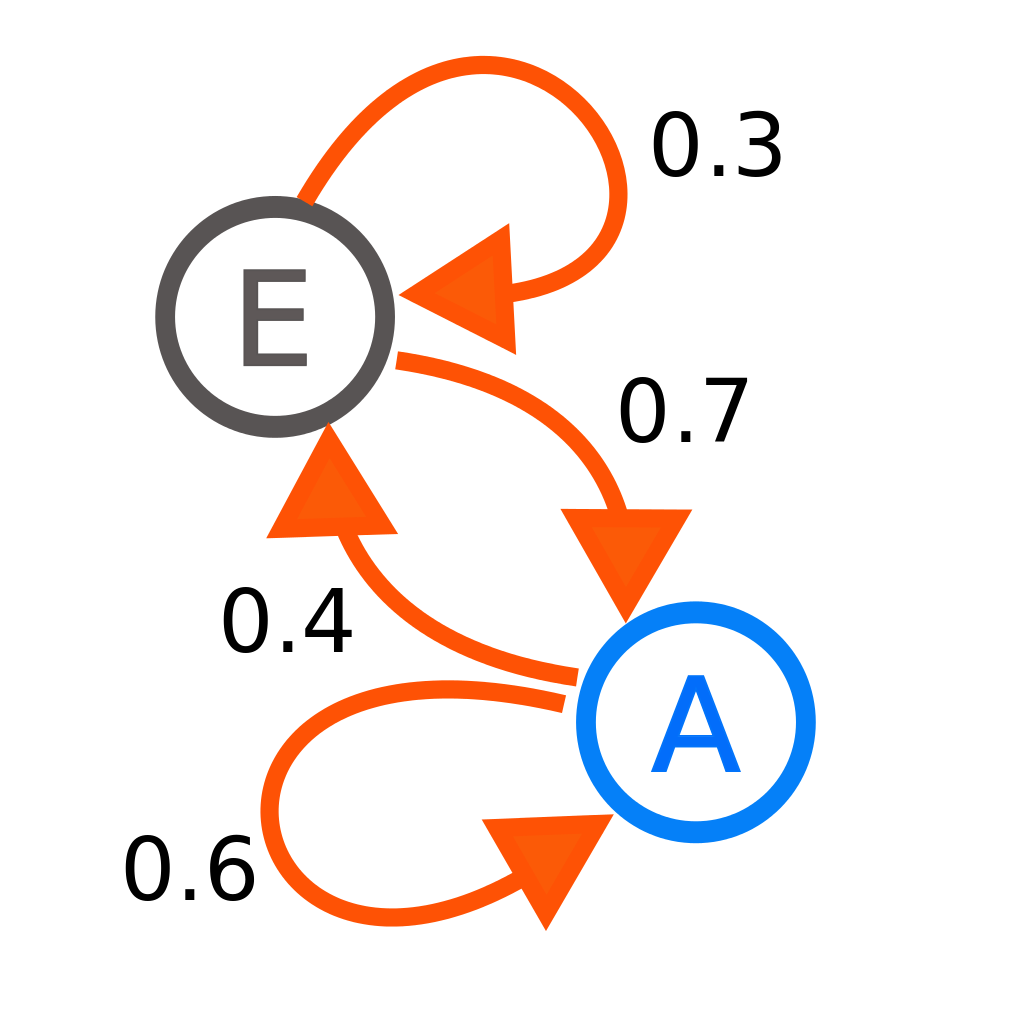
\includegraphics[width=0.25\linewidth]{images/markow-kette.png}}}%
    \qquad
    \subfloat[][]{\frame{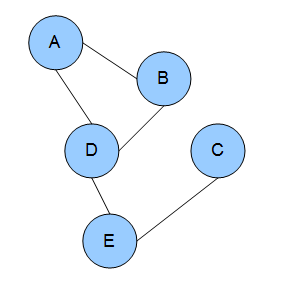
\includegraphics[width=0.25\linewidth]{images/Markov-netzwerk.png}}}%
    \caption{(a) Markow-Kette mit 2 möglichen Zuständen und deren Wahrscheinlichkeiten \cite{wiki:Markow-Kette}.
    Beispiel: Falls zustand $E$, dann gibt es eine $30\%$ Chance das der Zustand $E$ wieder Eintritt oder eine $70\%$ Chance das $A$ Eintritt.
    Falls wir den Zustand $A$ haben dann sind es $60\%$ für $A$ und $40\%$ für $E$. (b) Ein Markow-Netzwerk mit seinen Abhängigkeiten \cite{wiki:Markov_model}.
    Beispiel: $A$ ist abhängig von $B$ und $D$. $B$ von $A$ und $D$. $D$ von $A$, $B$ und $E$. $E$ von $D$ und $C$. Und zuletzt ist $C$ nur von $E$ abhängig.}%
\end{figure}

In einer Markow-Kette erster Ordnung hängt der Zustand nur vom vorhergehenden Zustand ab,
während bei einer Markow-Kette höherer Ordnung, somit ein Markov-Netzwerk, jeder Zustand von seinen Nachbarn in einer von mehreren Richtungen abhängt \cite{wiki:Markov_model}.
Ein Markow-Netzwerk kann als Feld oder Graph von Zufallsvariablen dargestellt werden,
wobei die Verteilung jeder Zufallsvariablen von den benachbarten Variablen abhängt, mit denen sie verbunden ist {(siehe Abbildung 2.4)}.

\section{Pyramid basierte Textur Synthese}

Bei der Pyramid-Methode wird das Verfahren der Bildpyramide verwendet.
Hierbei werden aus dem Input-Image mehrere Output-Images in verschiedenen Auflösungen mithilfe von Glättung und Downsampling generiert {(siehe Abbildung 2.5)} \cite{Heeger}.
\newline
Zudem wird ein Bildrauschen, \textit{(Noise-Image)} der i.d.R uniform weiß ist, verwendet.
Das Noise-Image wir dann durch von Histogram-Matching und der Image-Pyramid so verändert, das es dem Input-Image ähnlich ist.

\begin{figure}[H]
    \centering
    \subfloat[][]{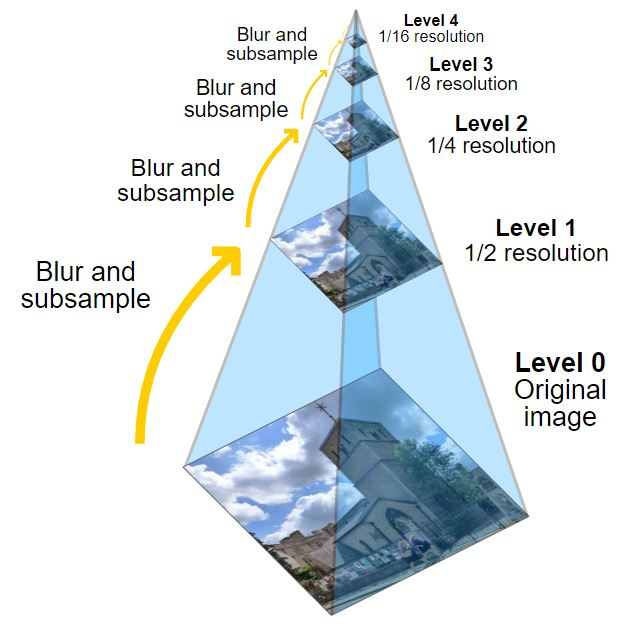
\includegraphics[width=0.4\linewidth]{images/pyramid.JPG}}%
    \caption{(a) Bildpyramide}%
\end{figure}

Histogram-Matching ist die Generalisierung des Punktoperators, mehr spezifisch, der Histogrammäqualisation.
Bei der Histogrammäqualisation {(auch Histogrammausgleich, Histogrammegalisierung oder Histogrammequalisierung genannt)}
werden die Kontraste von Grauwertbildern derart verbessert, sodass diese über eine bloße Kontrastverstärkung hinausgeht.
Dabei wird die Gleichverteilung mithilfe der Grauwertverteilung berechnet, damit der gesamte zur Verfügung stehende Wertebereich optimal ausgenutzt wird \cite{Lehmann2013}.
Bei dem Fall der Pyramid-Methode nimmt der Algorithmus ein Input-Image und bildet ein bestimmtes Histogramm, indem das Bild mit mehreren Nachschlagetabellen verarbeitet wird.
\paragraph{Die beiden Nachschlagetabellen Tabellen sind:}
\begin{itemize}
    \itemsep-0.5em
    \item Die kumulative Verteilungsfunktion \textit{(cumulative distribution function (CDF))} eines Bildes und
    \item die inverse kumulative Verteilungsfunktion eines Bildes.
\end{itemize} 

Die CDF ist eine Nachschlagetabelle, die das Intervall {[0,256]} auf das Intervall {[0,1]} abbildet.
Die inverse CDF ist eine Nachschlagetabelle, die von {[0, 1]} auf {[0, 256]} zurückführt.
Sie wird {(mit linearer Interpolation)} neu abgetastet,
sodass die Stichproben gleichmäßig auf dem Intervall {[0, 1]} verteilt sind \cite{Heeger}.
\newline
Während der Algorithmus weiter iteriert, beginnt das Noise-Image dem Input-Image zu ähneln wie wir Abbildung 2.6 {(c)} erkennen können.
Der Prozess stoppt, wenn eine ausreichende Ähnlichkeit erreicht ist oder eine festgelegte Anzahl von Iterationen erreicht wurde.

\begin{figure}[H]
    \centering
    \subfloat[][]{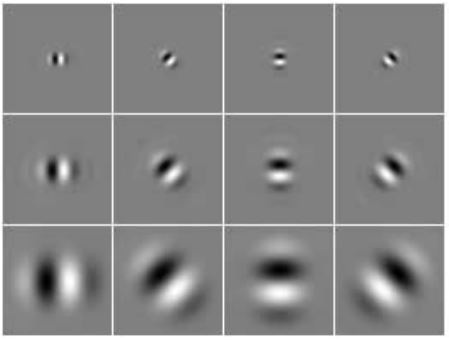
\includegraphics[width=0.2\linewidth]{images/pyramid-noise.JPG}}%
    \qquad
    \subfloat[][]{
\includegraphics[width=0.2\linewidth]{images/pyramid-input.JPG}}%
    \qquad
    \subfloat[][]{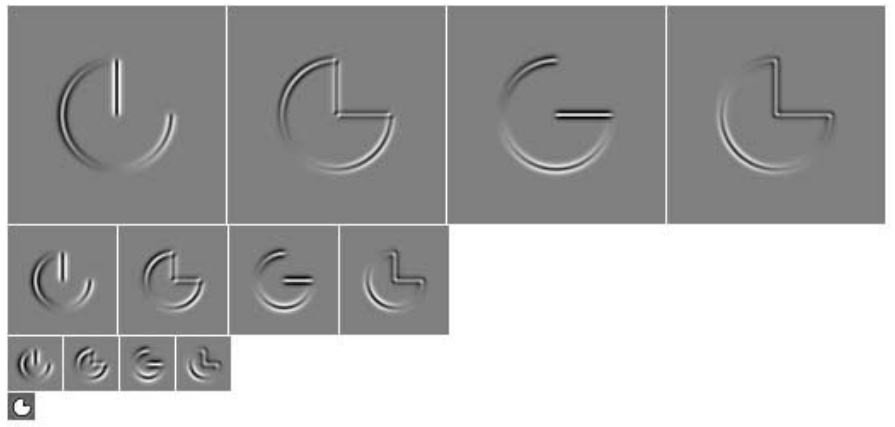
\includegraphics[width=0.3\linewidth]{images/pyramid-matching.JPG}}%
    \caption{(a) Projektion der Bildpyramide, (b) Input-Image, (c) Teilband-Bilder vom Input-Image.}%
\end{figure}

Die Pyramid-Methode ist eine weitere übliche Synthesemethode die, im Detail, sehr komplex ist und für das weitere Verständnis in dieser Arbeit keine Relevanz hat.
Daher wird sie nicht näher betrachtet.

\section{Patch basierte Textursynthese}

Die Patch basierte Textursynthese \textit{(auch Quilten genannt)} ist eine Erweiterung der Pixel basierten Textursynthese.
Hier werden statt einzelnen Pixeln ganze Felder \textit{(Patches)} verglichen und generiert {(siehe Abbildung 2.7)}.
Dabei werden die Patches mithilfe ihrer Nachbarn bestimmt und ausgewertet.
Dies hat zur Folge, dass sich die Qualität und die Geschwindigkeit des Algorithmus erhöht.

\begin{figure}[H]
    \centering
    \subfloat[][]{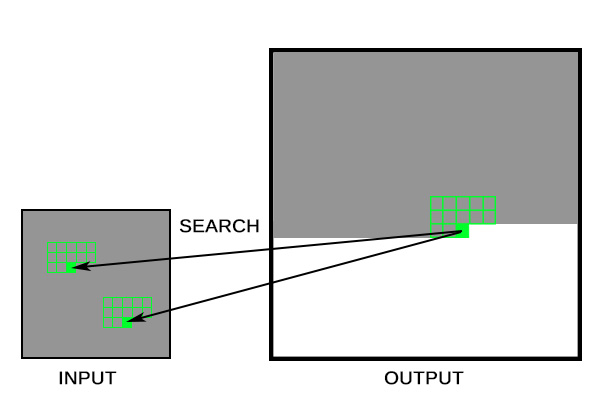
\includegraphics[width=0.45\linewidth]{images/Pixel-based.jpg}}%
    \qquad
    \subfloat[][]{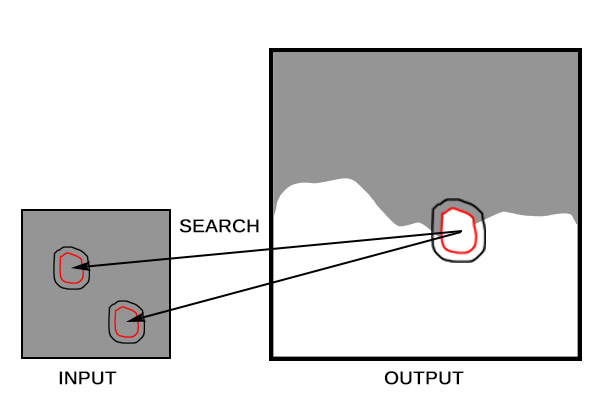
\includegraphics[width=0.45\linewidth]{images/Patch-based.jpg}}%
    \caption{(a) Pixel basiert, (b) Patch basiert.}%
\end{figure}

Ein Problem dieser Synthese im Vergleich zur Pixel basierten Synthese ist, dass sich hier die neuen Patches mit bereits vorhandenen Patches überschneiden.
Es gibt viele Methoden, um dieses Problem zu lösen {(siehe Abbildung 2.8)}.
Eine davon ist es, Patches mit verschiedenen Größen zu verwenden, damit die Konfliktbereiche zwischen den Patches durch das Phänomen der visuellen Maskierung
\textit{(Visual Masking)} reduziert werden.
Insbesondere bei stationären Texturen erreicht diese Methode gute Ergebnisse \cite{EfrosQuilt}.

\paragraph{Die Funktionsweise des Algorithmus nach D.Gomathi und Rajvi Shah:}

\begin{enumerate}
    \item Generierung des ersten Patches in der oberen-linken Ecke des Output-Images. Der Patch wird zufällig aus dem Input-Image ausgewählt.
    \item Von links-nach-rechts und von oben-nach-unten werden im Output-Image folgende Aufgaben ausgeführt.
    \begin{itemize}
        \item Auswahl des nächsten hinzuzufügenden Feldes aus dem Input-Image aus einem der am besten passenden Patches.
        \item Berechnen der Fehlerfläche zwischen diesem neuen Patch und seinem Überlappungsbereich mit bereits
        verarbeiteten Patches.
        \item Berechnen des Pfades mit den geringsten Kosten durch die Fehlerfläche, um die Patch-Grenze zu bestimmen, und fügen Sie dann den neuen Patch zum Output-Image hinzu {(siehe Abbildung 2.8 (c))}.
    \end{itemize}
\end{enumerate}

\begin{figure}[H]
    \centering
    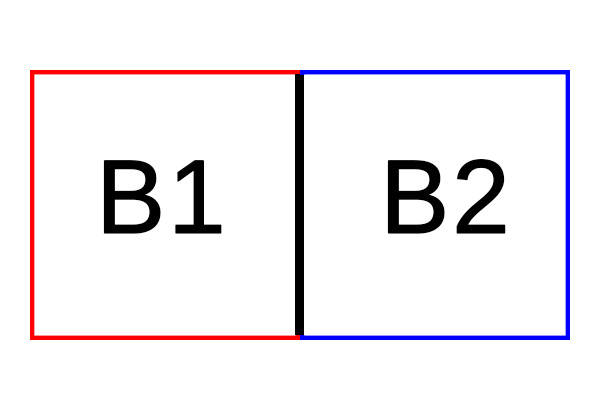
\includegraphics[width=0.25\linewidth]{images/Random-blocks.jpg}%
    \qquad
    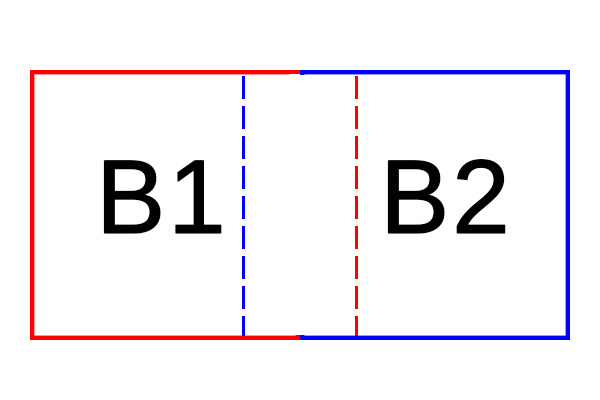
\includegraphics[width=0.25\linewidth]{images/overlap-blocks.jpg}%
    \qquad
    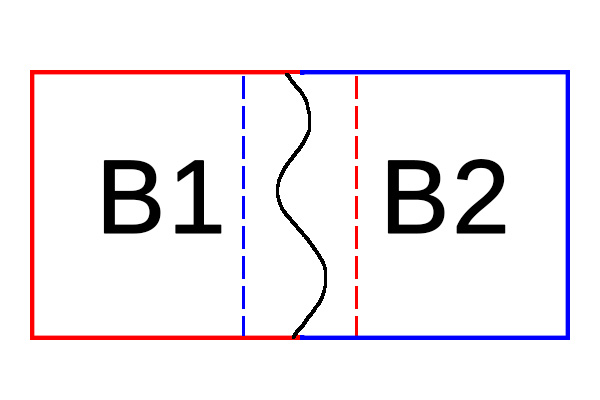
\includegraphics[width=0.25\linewidth]{images/minimum-boundary-blocks.jpg}%
    \qquad
    \qquad
    \subfloat[][]{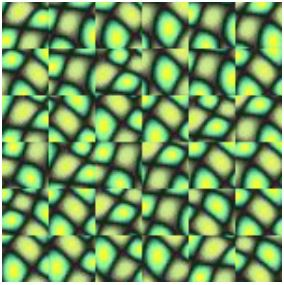
\includegraphics[width=0.25\linewidth]{images/texture-random-block.JPG}}%
    \qquad
    \subfloat[][]{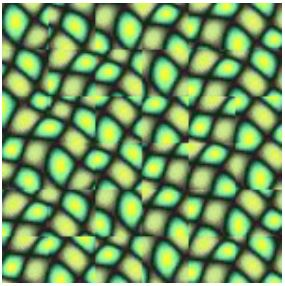
\includegraphics[width=0.25\linewidth]{images/texture-overlap-blocks.jpg}}%
    \qquad
    \subfloat[][]{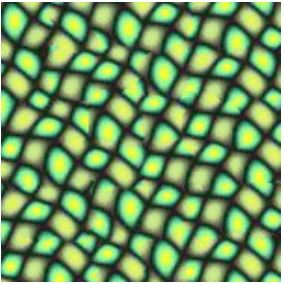
\includegraphics[width=0.25\linewidth]{images/texture-minimum-boundary-blocks.jpg}}%
    \caption{(a) Zufällige Patch Anordnung, (b) Patches eingeschränkt durch Nachbarn, (c) Minimal Fehler Randschnitt. Nach Alexei A. Efros und William T. Freeman \cite{EfrosQuilt}.}%
\end{figure}

\chapter{Wave-Function-Collapse}

Wichtig bei allen Textursynthesen ist,
dass die Muster des Output-Images immer lokal ähnlich oder gleich dem des Input-Images sein müssen.
Das wird größtenteils dadurch erzielt, dass aus dem Input-Image kleinere Subimages, Patches oder Pixel extrahiert werden.
Bei den Verfahren, bei denen die lokale Ähnlichkeit nicht 1-zu-1 bzw. pixelgenau stattfindet,
werden die Pixel und deren Farbwert oft nach Grundlage der Abstandsmetrik {(z.B. dem euklidischen Abstand von Pixelfarbvektoren)} beurteilt.
Solche Verfahren finden meistens in der visuellen Computergrafik Anwendung.
Diese Methodiken haben große Nachteile im Gegensatz zu Algorithmen, bei denen das lokale Muster des Outputs pixelgenau dem Input-Image gleicht.
Gerade für PCG {(Procedural-Content-Generation)} kann die Pixelgenauigkeit von großem Nutzen sein, da dadurch Abgrenzungen der Pixel innerhalb des Output-Images klar definiert sein können 
\cite{Karth2017WaveFunctionCollapseIC}.
Von allen oben beschriebenen Textursynthese-Methoden ist der WFC der Patch basierten Methode am ähnlichsten.
\newline
Gumin hat von Paul Merrell's Arbeit inspirieren lassen, obwohl dieser sich hauptsächlich mit der Generierung von 3D-Modellen beschäftigte.
Bei Merrell's Verfahren werden die Modelle mithilfe von bereits erstellten Bausteinen zusammengesetzt.
Das ist dahingehen von Vorteil, da sich in vielen Textursynthesen die Übergänge der Pixel vermischen und sich somit Artefakte bilden können.
Dieses Verhalten ist bei WFC und dem Verfahren von Paul Merrell nicht möglich, da es sich um eine diskrete Synthese handelt.
Jedes lokale Muster ist immer im Input wiederzufinden {(siehe Abbildung 3.1)} \cite{Karth2017WaveFunctionCollapseIC, merrell2009model, Gumin_Wave_Function_Collapse_2016}.

\begin{figure}[H]
    \centering
    \subfloat[][]{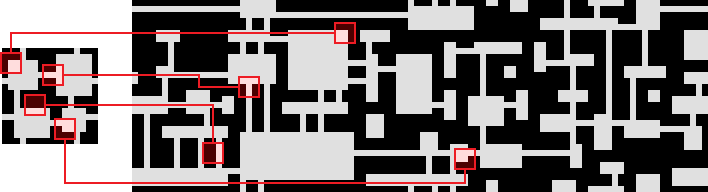
\includegraphics[width=1\linewidth]{images/wfc-pattern.png}}%
    \caption{(a) WFC generiertes Muster.}%
\end{figure}

\section{Constraint-Satisfaction-Problem {(CSP)}}

Der WFC von Gumin ist lose an der Quantenmechanik angelehnt.
Das liegt daran, dass bei der Synthese von WFC in jeder Zelle des $N\times N$ Output-Images theoretisch jedes Muster / jeder Pixelwert vorkommen kann, bevor dies final festgelegt werden.
Dieser Zustand nennt sich \textit{Superposition} {(siehe Abbildung 3.2)}.
Jede Zelle hat mehrere Eigenwerte \textit{(eigenstates)} und somit auch eine maximale Entropie bzw. einen maximalen Informationsgehalt.
Auch hat jede Zelle bestimmte Regeln, die sich aus deren Nachbarzellen ergeben und erfüllt werden müssen.
Denn nicht jede Zelle kann an jeder Position auftauchen, sobald bereits eine Zelle ein Eigenwert erhält
{(siehe Patch basierte Textursynthese. Nicht jeder Patch kann an einer beliebigen Position sein,
da sie sich den Nachbarn anpassen müssen, damit die Synthese nahtlos ist.)}
Sobald eine Zelle bekannt wird \textit{(Observation)} und nur einen Eigenwert besitzt,
wird die Entropie aller anderen Zellen angepasst.
\say{Nach dieser Auffassung ist der "collapse" der Wellenfunktion kein
physikalischer Prozess und spiegelt lediglich eine Aktualisierung unserer Informationen über das System wider.} \cite[S.5, 2.2 The wave function]{Zinkernagel_2016}
Da der WFC Algorithmus genau auf diese Art und Weise die Synthese durchführt,
kann der WFC auch als Löser für solche Bedingungserfüllungsprobleme \textit{(Constraint-Satisfaction-Problem)} verwendet werden.\par

Grundsätzlich beschreiben CSP's Gruppen von Objekten, denen Variablen zugeteilt sind.
Diesen Objekten sind Regeln, sogenannte \textit{(constraints)} auferlegt, die erfüllt werden müssen.
Jeder dieser Objekte hat zu Beginn eine Superposition und kann somit grundsätzlich jeden Wert enthalten.
Die Aufgabe von Algorithmen zum Lösen von CSP's \textit{(solver)} ist es einen Zustand \textit{(State)} zu finden,
in dem alle constraints erfüllt sind und jedem Objekt nur noch ein Wert zugeordnet ist \cite{Lecoutre2009ConstraintNT}.
Solche Probleme finden sich oft bei der Künstlichen Intelligenz und bei Operations Researchs wieder.
Im Fall von WFC sind die Objekte, denen die Variablen zugeteilt sind, die einzelnen Bereiche im Output-Image.
Jedem dieser Bereiche muss ein lokales Muster aus dem Input zugeordnet werden.
Immer, wenn einem Bereich ein Wert zugeordnet wird, werden auch die benachbarten Bereiche damit beeinflusst \textit{(Propagation)}.
Der Gesamtprozess, wenn sich eine Gruppe aus Superpositionen mit mehreren Eigenwerten zu einem einzelnen Eigenwert aufgrund von Interaktion mit der Außenwelt \textit{(Observation)} reduziert,
nennt sich Wave-Function-Collapse \cite{Zinkernagel_2016}.
Während dem Prozess einen gültigen State für das CSP zu finden, so kann es immer Situationen geben, in dem es mehrere gültige Optionen / Eigenwerte für ein Objekt gibt.
Wenn eine solche Situation auftritt, dann haben verschiedene Solver verschiedene Lösungsansätze.
Einige Algorithmen wählen zufällig einen der möglichen Werte aus den momentan zulässigen Optionen.
Bei diesem Ansatz kann es sein, dass der Algorithmus nicht auf einen Zustand kommen kann, bei dem alle constraints erfüllt werden können.
In so einem Fall gibt es Rücksetzverfahren \textit{(Backtracking)}, bei dem der Algorithmus zu seinem letzten Ergebnis zurückfällt und einen anderen Wert für die Variable setzt,
um den ungültigen Zustand zu verlassen und diesen neu zu berechnen.
Andere Algorithmen verwenden zusätzliche Heuristiken abgesehen von den bereits bekannten constraints, um die Möglichkeit eines ungültigen Zustandes zu reduzieren \cite{Karth2017WaveFunctionCollapseIC}.
\pagebreak

\subsection{CSP-Beispiel an Sudoku}
Es gibt viele verschiedene CSP Probleme in der Wissenschaft.
Eines der bekanntesten Probleme, welches Menschen nahezu täglich unbewusst lösen, ist Sudoku.
Sudoku ist ein CSP welcher am besten auch die Funktionsweise von Gumin's WFC aufzeigt, da die Constraints der Probleme sehr ähnlich sein können.
Wenn ein Sudoku Feld ohne initiale Zahlen betrachtet \textit{(unobserved)} wird, kann in jedem einzelnen Objekt,
in diesem Fall auch Zelle, theoretisch jede Zahl vorhanden sein \textit{(Superposition)} \cite{boris}.

\begin{figure}[H]
    \centering
    \subfloat[][]{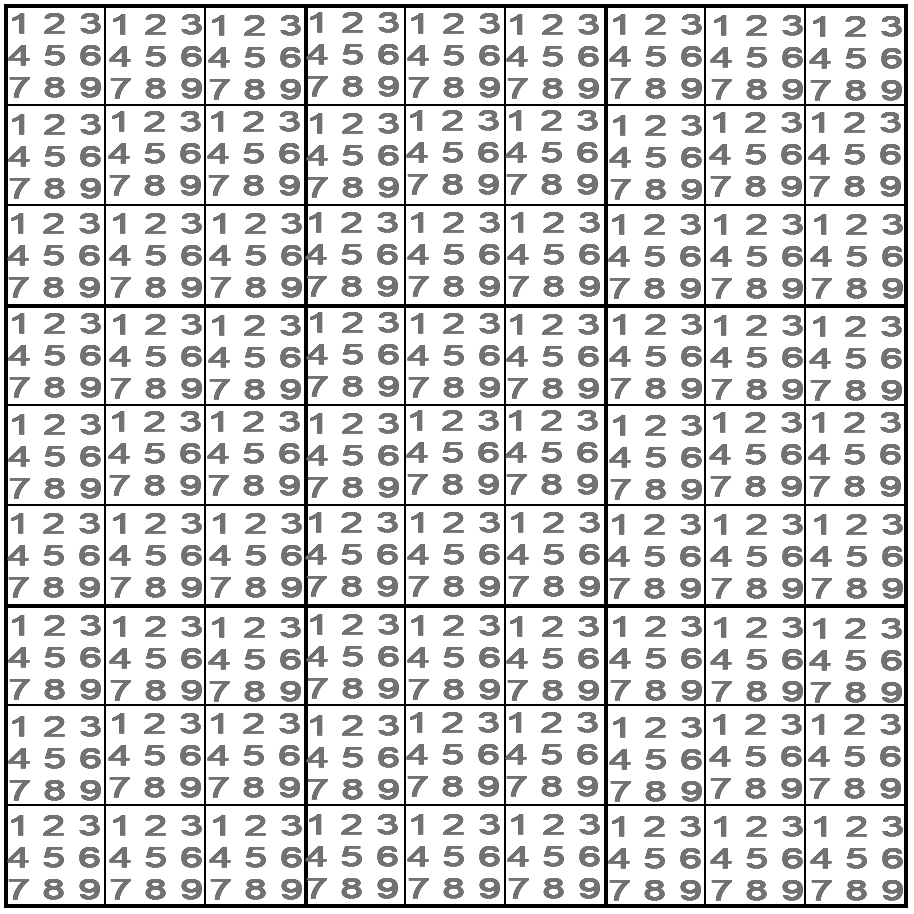
\includegraphics[width=0.9\linewidth]{images/sudoku-superposition.png}}%
    \caption{(a) Sudoku Feld unbeobachtet in einer Superposition.}%
\end{figure}

\paragraph{Die Regeln \textit{(constraints)} dieses CSP sind wie folgt:}
\begin{enumerate}
    \item Jede Zeile, Spalte und jedes Quadrat {(je 9 Felder)} muss mit den Zahlen 1-9 ausgefüllt werden.
    \item Keine Zahl innerhalb der Zeile, Spalte oder des Quadrats darf sich wiederholen.
\end{enumerate}

In Abbildung 3.3 erkennen wir den ersten Schritt der initiale \textit{Observation}, dabei wird das erste Feld mit seinen vielen Eigenwerten auf einen festen Wert kollabiert.
Dadurch treten für die benachbarten Zellen die Constraints ein, die bestimmen, welche Werte diese noch einnehmen können \cite{boris}.

\begin{figure}[H]
    \centering
    \subfloat[][]{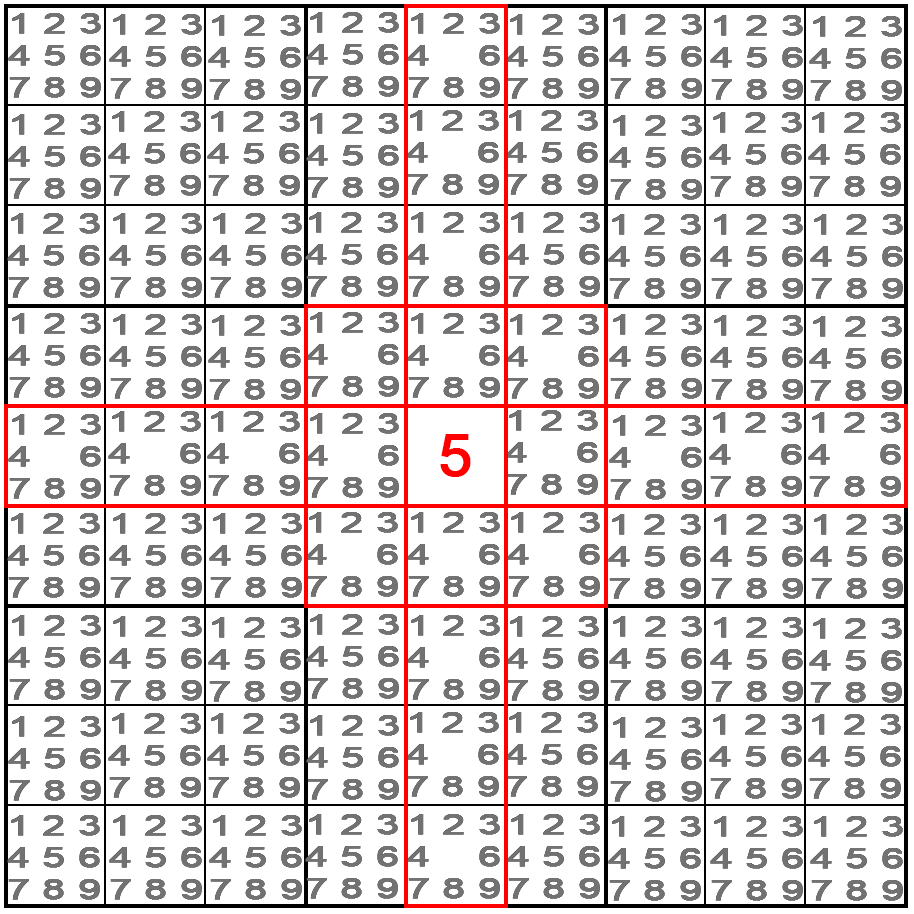
\includegraphics[width=0.9\linewidth]{images/sudoku-observed.png}}%
    \caption{(a) Sudoku Feld mit dem ersten Input.}%
\end{figure}

Nach dem ersten Input reduziert sich die Entropie aller Zellen in jeder betroffenen Zeile,
Spalte und Quadrat bzw. ihre Anzahl an möglichen Eigenwerten reduziert sich.
Als nächsten Schritt könnte jetzt eine beliebige Zelle ausgewählt und diese auf einen ihrer zufälligen möglichen Eigenwerte gesetzt werden.
Allerdings besteht dabei immer die Möglichkeit, dass der Prozess einen Zustand erreicht, an dem kein gültiger Zustand erreicht werden kann.
Um die Wahrscheinlichkeit dieses Szenarios zu reduzieren, können Heuristiken eingesetzt werden,
um eine Auswahl zu treffend die zu einem gültigen Endzustand führt.
In diesem Fall wird eine Zelle ausgewählt, die bereits eine sehr niedrige Anzahl an möglichen Eigenwerten hat, bzw. eine sehr niedrige Entropie besitzt.
Dadurch ist die Wahrscheinlichkeit geringer, dass eine Zelle auf einen nachteiligen Wert gesetzt wird,
der später zu einem ungültigen Endzustand führt {(siehe Abbildung 3.4)} \cite{boris}.
\footnote[2]{Dies ist nicht zwingend der fall für WFC. Dazu später mehr.}

\begin{figure}[H]
    \centering
    \subfloat[][]{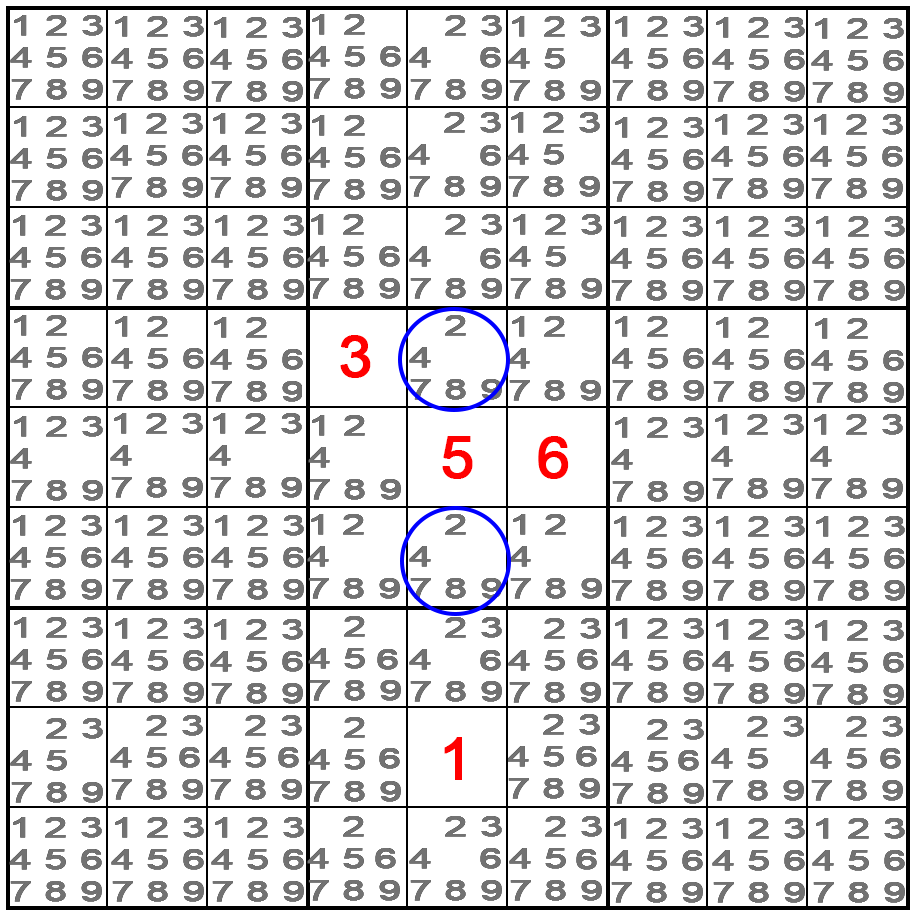
\includegraphics[width=0.9\linewidth]{images/sudoku-observed-heurisitk.png}}%
    \caption{(a) Sudoku Feld mit mehreren festgelegten Zellen. Blau markierte Zellen sind mögliche Kandidaten für nächsten Zyklus.}%
\end{figure}

Dieser Zyklus wiederholt sich so lange, bis alle Zellen ausgefüllt sind.

\section{WFC und die Model Synthese}

Wie bereits erwähnt, wurde der WFC Algorithmus von Gumin durch Paul Merrell's diskreter Model Synthese inspiriert.
Die Model Synthese wurde durch die Patch basierte Textursynthese inspiriert und ist, wie WFC, ebenfalls ein Lösungsalgorithmus für CSP's.
\newline
Eine Textursynthese kann in vielen Bereichen angewendet werden.
Ausgenommen, wenn im Input-Image feste Strukturen vorkommen oder eine Synthese im 3D-Raum generiert werden soll,
dann sind nicht alle Synthesemethoden anwendbar.
Diese Probleme wollte Paul Merrell mit seiner Model Synthese lösen \cite{merrell2009model}.

\begin{figure}[H]
    \centering
    \subfloat[][]{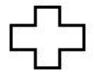
\includegraphics[width=0.1\linewidth]{images/input-shape.JPG}}%
    \qquad
    \subfloat[][]{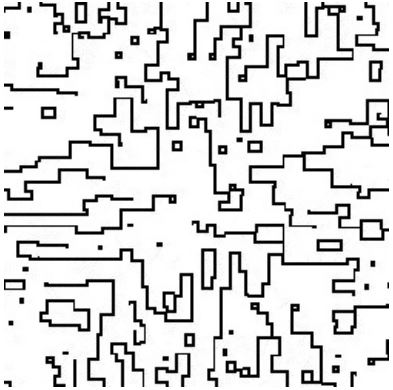
\includegraphics[width=0.25\linewidth]{images/Efros-Leung-1999.JPG}}%
    \qquad
    \subfloat[][]{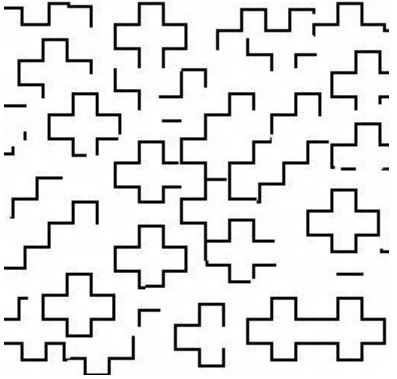
\includegraphics[width=0.25\linewidth]{images/Kwatra-2005.JPG}}%
    \caption{(a) Input Struktur, (b) Alexei A. Efros and Thomas K. Leung 1999, (c) Kwatra et al., 2005 \cite{merrell2009model}.}%
\end{figure}

Viele dieser gängigen Textursynthesen scheitern an Strukturen, da diese Aufgelöst werden nicht als geschlossenes Objekt erkannt werden.
In Abbildung 3.5 sind genannte Schwachstellen von den anderen Textursynthesen klar erkennbar.
\newline
Paul Merrell erkannte, dass viele natürliche und künstliche Objekte aus sich immer wiederholenden Komponenten bestehen.
Dies führte zu dem Ansatz, mit ganzen Komponenten, statt mit einzelnen Pixel zu arbeiten.
Dadurch können neue Objekte sowohl im 2D als auch im 3D-Raum generiert werden {(siehe Abbildung 3.6 (c))} \cite{merrell2009model}.

\begin{figure}[H]
    \centering
    \subfloat[][]{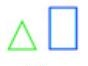
\includegraphics[width=0.1\linewidth]{images/Beispiel-textur.JPG}}%
    \qquad
    \subfloat[][]{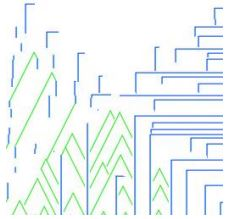
\includegraphics[width=0.25\linewidth]{images/Efros-Leung-textur.JPG}}%
    \qquad
    \subfloat[][]{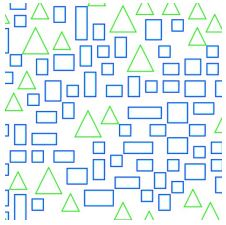
\includegraphics[width=0.25\linewidth]{images/Paul-merrells-Model-synthese.JPG}}%
    \caption{(a) Input Struktur, (b) Alexei A. Efros and Thomas K. Leung, (c) Paul Merrell Model Synthese \cite{merrell2009model}.}%
\end{figure}

Anders als bei Sudoku, gilt bei der Model Synthese jedoch die Regel der Adjazenz-Bedingung \textit{(adjacency constraint)}.
Die Adjazenz-Bedingung stellt sicher, dass alle Teile des Modells nahtlos zusammenpassen und dass das neue Modell dem Input ähnlich ist {(siehe Abbildung 3.7)}.

\begin{figure}[H]
    \centering
    \subfloat[][]{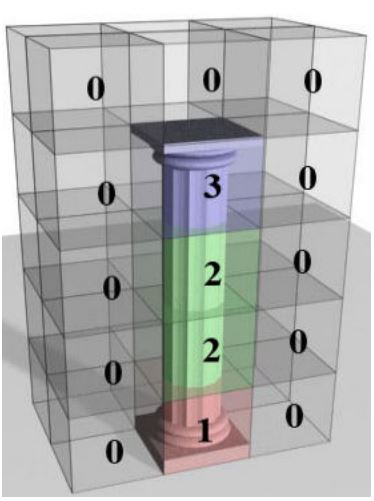
\includegraphics[width=0.25\linewidth]{images/model-divided.JPG}}%
    \qquad
    \subfloat[][]{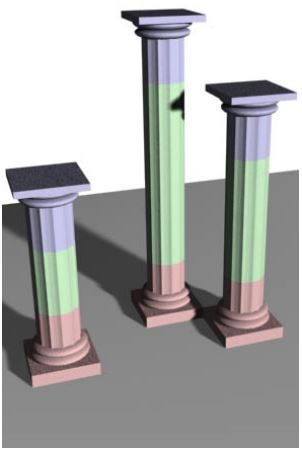
\includegraphics[width=0.25\linewidth]{images/seamless-model.JPG}}%
    \qquad
    \subfloat[][]{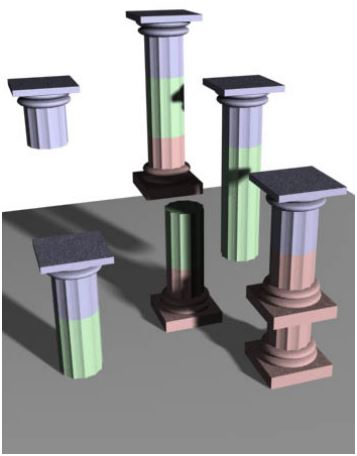
\includegraphics[width=0.25\linewidth]{images/modell-conflicts.JPG}}%
    \caption{(a) 3D-Modell in Komponenten aufgeteilt, (b) Komponente nahtlos zusammengesetzt, (c) Komponente halten Adjazenz-Bedingungen nicht ein \cite{merrell2009model}.}%
\end{figure}

\paragraph{Der grundsätzliche Ablauf der Model Synthese im 2D-Raum ist wie folgt:}

\begin{enumerate}
    \itemsep-1em
    \item Erstelle Module {(siehe Abbildung 3.8 (a))}.
    \item Wähle eine Zelle unter eventueller Berücksichtigung von Heuristiken.
    \item Kollabiere die Zelle auf einen Eigenwert.
    \item Errechne neue mögliche Eigenwerte der benachbarten Zellen \textit{(Propagation)}  {(siehe Abbildung 3.8 (b))}.
    \item Wiederhole Schritte 2 bis 4.
\end{enumerate}

\begin{figure}[H]
    \centering
    \subfloat[][]{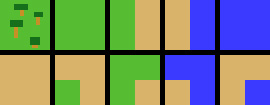
\includegraphics[width=0.4\linewidth]{images/modules-cells.png}}%
    \qquad
    \subfloat[][]{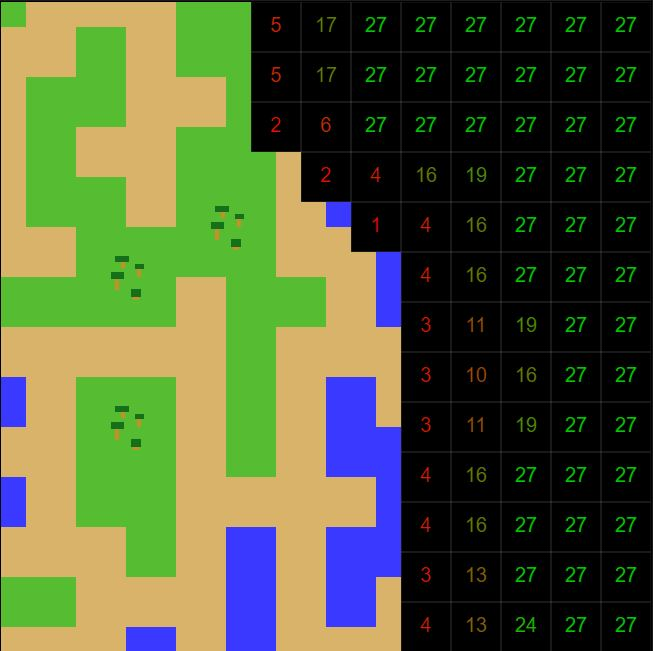
\includegraphics[width=0.5\linewidth]{images/collapse-cells.JPG}}%
    \caption{(a) Module, (b) Möglicher Output mit möglichen Optionen pro Zelle.}%
\end{figure}

An diesem Punkt ist es wichtig zu erwähnen,
dass es sich hierbei bereits um das \say{Simple Tile Model} des WFC Algorithmus handelt.

\subsection{Unterschiede zwischen WFC und Model Synthese}

Tatsächlich ist der WFC Algorithmus von Gumin und die Model Synthese von Merrell, in der Ausführung der oben genannten Schritte, nahezu identisch.
Der Unterschied zwischen den beiden Algorithmen besteht lediglich in der Implementierung der einzelnen Schritte, sowie in zusätzlichen Optimierungen.
Laut Paul Merrell gibt es mehrere Unterschiede in der Implementierung.
Ein Unterschied ist die Reihenfolge der Auswahl der nächsten Zelle.
Während WFC nach der niedrigsten Entropie Heuristik seine Zelle auswählt,
wählt die Model Synthese nach der Scanline-Methode, in der erst Reihe für Reihe durch das Modell / Bild iteriert wird, seine Zellen aus.
Die Zellenauswahl von WFC verursacht mehr Fehlerzustände bei großen Output-Images als die von Paul Merrell's Model Synthese.
Auch die Komplexität des Inputs kann dazu beitragen, dass WFC nicht zu einem Ergebnis kommt.
Obwohl das ebenfalls der Fall bei Merrell's Implementierung ist, ist es bei der Model Synthese wesentlich wahrscheinlicher, dass ein gültiges Ergebnis zustande kommt,
da die Model Synthese Fehlerbehandlungen besitzt, die bei WFC fehlen.
\newline
Einer dieser Fehlerbehandlungen ist die Blockweise Generierung vom Output-Image.
In der Model Synthese wird der Output blockweise generiert und nicht komplett in einem Durchgang.
Das ist für die Generierung von großen Outputs, vor allem bei 3D-Modellen, von großer Bedeutung, da dadurch die Fehlerquote bei einigen Inputs signifikant reduziert wird.
WFC teilt sein CSP nicht in kleinere Blöcke auf, da der Output von WFC in der Regel kleiner ist, und die Verarbeitung im 2D-Raum wesentlich einfacher.
Dennoch kann das WFC von einer solchen Implementierung profitieren, wenn man WFC im 3D-Raum verwenden möchte oder größere Outputs erzielen möchte \cite{merrell2018compare}.

\begin{table}[H]
    \centering
    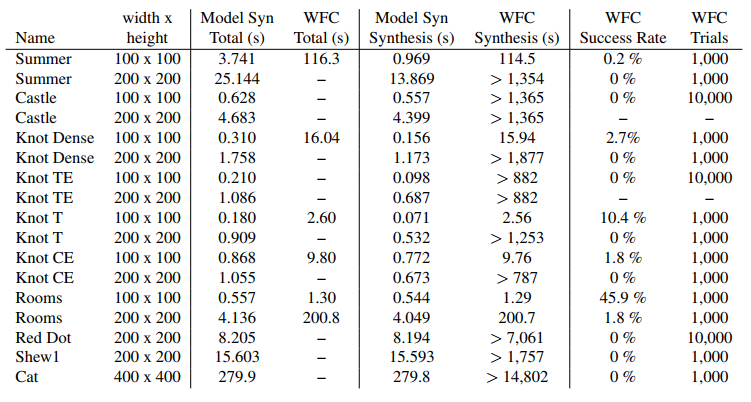
\includegraphics[width=1\linewidth]{images/timing-and-success-comparison.png}%
    \caption{Paul Merrell's Vergleich zwischen WFC und seiner Model Synthese \cite{merrell2018compare}.}%
\end{table}

In Tabelle 3.1 wird die Erfolgsquote sowie die benötigte Zeit zur Generierung der genannten Inputs verglichen.
Die Resultate können in Abbildungen 5.1 bis 5.4 betrachtet werden.
Der WFC kommt aufgrund der Größe des Outputs als auch der Komplexität des Inputs nicht immer auf gültige Ergebnisse.
Es wird deutlich, dass die Model Synthese fast immer zu einem erfolgreichen Resultat kommt,
da die Größe der einzelnen Blöcke einfach reduziert werden kann, um die Erfolgsquote zu steigern \cite{merrell2018compare}.\par

Neben weiteren Unterschieden, wie der Laufzeit und der Erweiterbarkeit der beiden Algorithmen, gibt es noch einen weiteren Unterschied den Gumin's WFC implementiert.
Das sogenannte Overlapping Model, das in der Originalversion von Gumin vorkommt, ist das, was WFC initial bekannt gemacht hat.

\pagebreak

\subsection{Simple Tile Model und Overlapping Model}

Anders als bei dem Simple Tile Model von WFC, bei dem einzelne Module für die Synthese bereitgestellt werden,
benötigt das Overlapping Model von WFC ein komplettes Input-Image, das daraufhin analysiert wird.
Aus dieser Analyse werden die Module automatisch generiert.
Zudem haben sich die Module bei dem Simple Tile Model nicht überschnitten, wie es bei dem Overlapping Model der Fall ist.
Das hat den Vorteil, dass die Module direkt aus dem Input errechnet werden können {(siehe Abbildung 3.9 und 3.10)}.
Zudem kann der Output dem Input ähnlicher sein, da die Module näher aneinander liegen \cite{merrell2018compare}.

\begin{figure}[H]
    \centering
    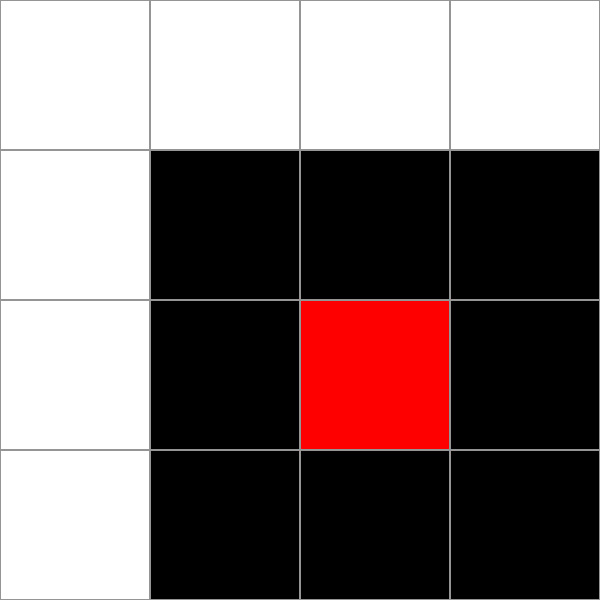
\includegraphics[width=0.5\linewidth]{images/red-maze.jpg}%
    \caption{$4\times 4$ Pixel Red-Maze Beispiel Input \cite{Karth2017WaveFunctionCollapseIC}.}%
\end{figure}


\begin{figure}[H]
    \centering
    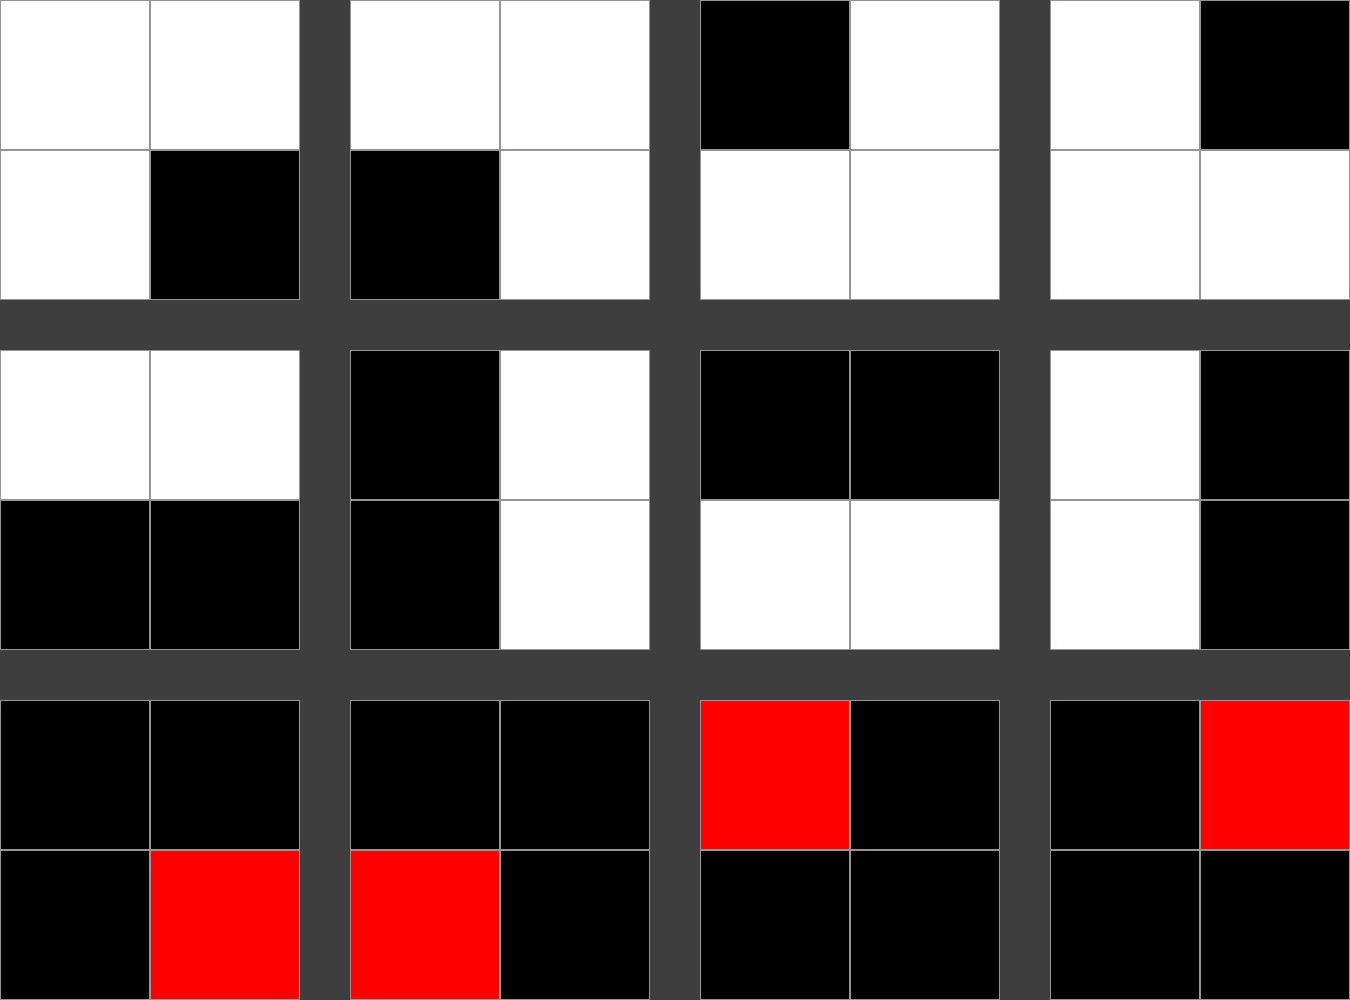
\includegraphics[width=0.5\linewidth]{images/red-maze-modules.jpg}%
    \caption{Alle Red-Maze Module der Größe $N = 2$ mit Spiegelungen und Rotationen \cite{Karth2017WaveFunctionCollapseIC}.}%
\end{figure}

\newpage

Bei einem $N = 2$ Patch gibt es insgesamt 9 verschiedene Möglichkeiten, wie diese übereinander liegen können {(siehe Abbildung 3.11)}.
{(Wenn $N = 3$ dann $(2(N - 1) + 1)^2 = 36$ offsets.)}
Der WFC Algorithmus legt eine Indexstruktur an, die die Möglichkeiten beschreibt, wie die Muster nebeneinander platziert werden können.
Bei diesem Model enthält der Index die vorberechnete Anzahl an gültigen Module, die an einem anderen Index mit $x,y$-Offset platziert werden dürfen. 
Bei dem in Kapitel 3.1.2 beschriebenen Sudoku-Beispiel, könnte dies angewendet werden,
indem jede Zelle im Feld eine bestimmte $x,y$ Koordinate besitzt, damit durch diese iteriert werden kann.
Sobald ein Feld einen Wert besitzt, werden in allen benachbarten Zellen Module entfernt, die nicht nutzbar sind \cite{Karth2017WaveFunctionCollapseIC}.

\begin{figure}[H]
    \centering
    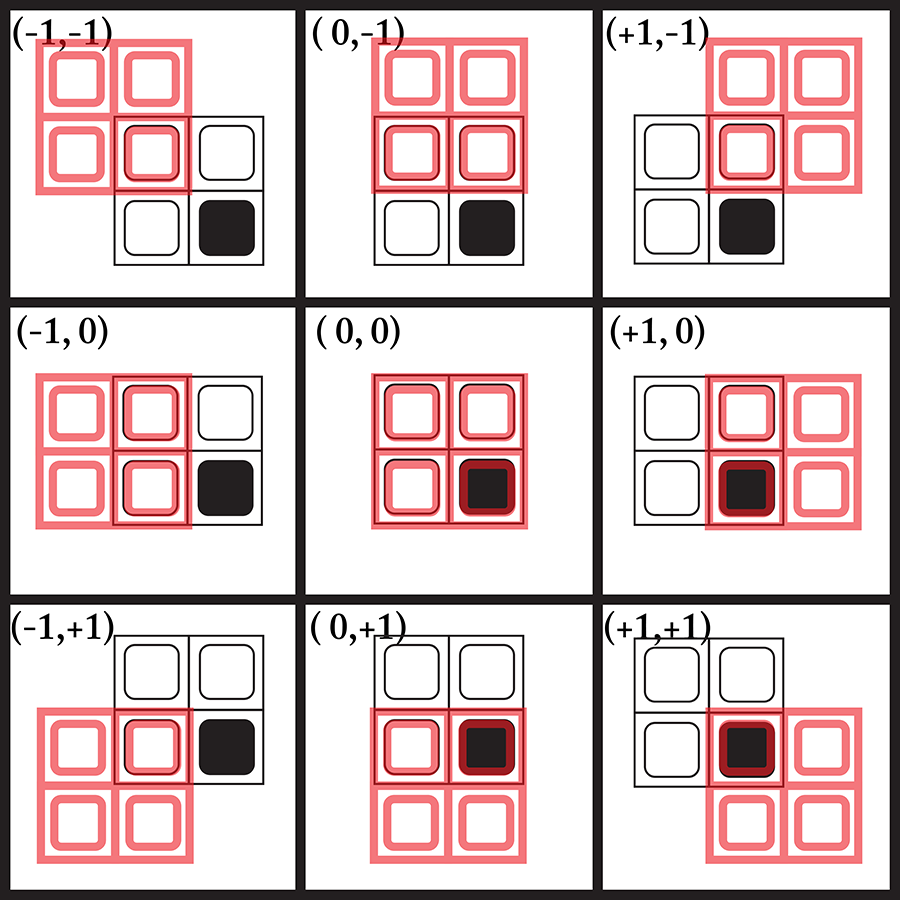
\includegraphics[width=0.5\linewidth]{images/red-maze-offset.png}%
    \caption{Die 9 Möglichkeiten wie die Module übereinander liegen können \cite{Karth2017WaveFunctionCollapseIC}.}%
\end{figure}

In Abbildung 3.12 erkennen wir einen Ausschnitt einer einzelnen Zelle mit allen möglichen Module, die an ihren benachbarten $x,y$-Offsets erlaubt sind, dargestellt.
Dabei ist bei einem Offset mit den Werten $(0,0)$ {(kein Offset)} immer nur der betrachtete Patch nutzbar {(bzw. die Zelle mit bereits einzelnem Eigenwert)}.
Als Beispiel Offset $(-1,0)$. Da sind nur Module möglich, die Rechts zwei weiße Pixel besitzen damit sie sich nahtlos mit den zwei weißen Pixel bei $(0,0)$ überlappen können \cite{Karth2017WaveFunctionCollapseIC}.

\begin{figure}[H]
    \centering
    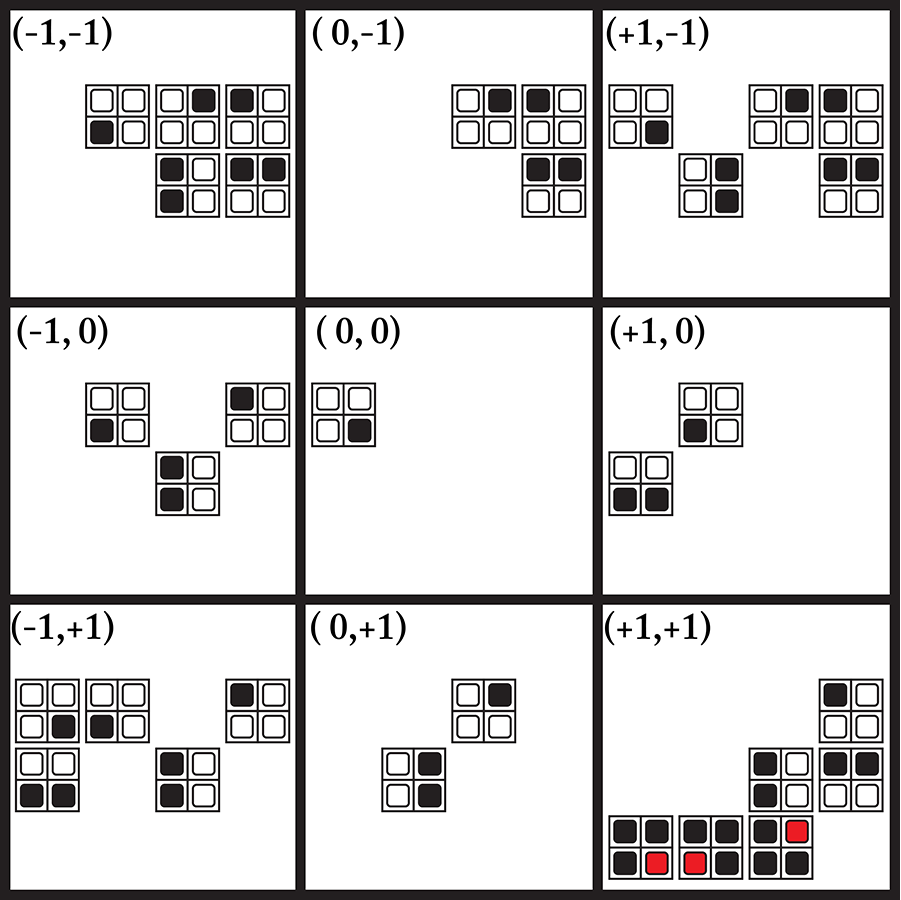
\includegraphics[width=0.5\linewidth]{images/red-maze-offset-example.png}%
    \caption{Ausschnitt einer Zelle. Von 12 möglichen Modulen sind nur die gültigen Optionen für die benachbarten Zellen mit $x,y$-Offset möglich \cite{Karth2017WaveFunctionCollapseIC}.}%
\end{figure}

In diesem Beispiel wurden mit $N = 2$, dies Entspricht in diesem Fall einer Fenstergröße von zwei Pixeln, die einzelnen Module aus dem Input generiert.
Die Fenstergröße wird von dem Entwickler festgelegt und hat direkten Einfluss auf den Output.
Falls $N = 1$ gesetzt wird, und somit nur einzelne Pixel verarbeitet werden, dann befinden wir uns wieder beim Simple Tile Model.
Allerdings funktioniert $N = 1$ in diesem Fall nicht, da jeder Pixel zu einem Patch wird, da diese nicht mehr überlappt werden können,
es sei denn $N = 1$ repräsentiert eine Menge an Pixeln.
Bei einer zu kleinen Fenstergröße kann es vorkommen, dass der Output nicht dem Input ähnelt.
Bei einer zu großen Fenstergröße kann der Output dem Input zu ähnlich sein, da ganze Gruppen von Strukturen kopiert und eingefügt werden.
Daher hat die Wahl der Größe, Einfluss auf das Ergebnis {(siehe Abbildung 3.13 und 3.14)}.

\begin{figure}[H]
    \centering
    \frame{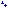
\includegraphics[width=0.25\linewidth]{images/input-example-overlapping.png}}%
    \caption{Beispiel Input-Image ($8\times8$ Pixel) für ein Overlapping Model.}%
\end{figure}

\begin{figure}[H]
    \centering
    \subfloat[][]{\frame{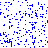
\includegraphics[width=0.25\linewidth]{images/output-overlapping-n2.png}}}%
    \qquad
    \subfloat[][]{\frame{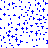
\includegraphics[width=0.25\linewidth]{images/output-overlapping-n3.png}}}%
    \qquad
    \subfloat[][]{\frame{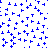
\includegraphics[width=0.25\linewidth]{images/output-overlapping-n4.png}}}%
    \caption[]{(a) Output mit $N = 2$, (b) Output mit $N = 3$, (c) Output mit $N = 4$. Beispiele generiert mit Kchapelier's Overlapping Model.\footnote[3]{\url{http://www.kchapelier.com/wfc-example/overlapping-model.html}}}
\end{figure}

Es ist wichtig anzumerken, dass viele der hier gezeigten Texturen auch mit aktuellen Textursynthese-Algorithmen generiert werden können.
Der Vorteil von Model Synthese und WFC im Vergleich zu anderen Synthesen ist, dass der generierte Content auch Interaktiv genutzt werden kann,
da wir bei diesen Verfahren der Entwickler die gesamte Kontrolle über die lokalen Muster des Outputs hat und das Endergebnis alle auferlegten Constraints erfüllt.
Gerade der Simple Tile Model Algorithmus bietet sich deswegen für PCG an, da der Entwickler die Kontrolle über die einzelnen Module hat,
die dann für das Output zusammengesetzt werden.
Dadurch, und das keine unvorhersehbaren Artefakte entstehen können, qualifiziert den WFC für den Einsatz in der Spiele-Entwicklung.
Wird statt einem lokalen und stationären Input {(siehe Abbildung 2.2)} bspw. ein Foto verwendet,
dann würden die anderen Synthesemethoden, im Gegensatz zur Model Synthese und WFC, passendere Ergebnisse liefern, sofern diese mit der Verwendung von KI dafür ausgelegt sind.
Es sei erwähnt, dass der Input für WFC nicht \say{strikt} eine Textur wie in Abbildung 2.2 {(b)} sein muss.
Diese Texturen sollten allerdings Selbstähnlichkeit besitzen und nur wenige unterschiedliche Pixelfarben verwenden.
Bereits ein Tag nach der Veröffentlichung von Gumin's WFC am 30. September 2016 haben viele Entwickler begonnen mit diesem Algorithmus zu experimentieren \cite{Karth2017WaveFunctionCollapseIC}.
Ein Grund für die große Beliebtheit von Gumin's WFC Algorithmus ist neben der bereits erwähnten Pixelgenauigkeit und die damit einhergehende Möglichkeit den Output Interaktiv zu nutzen,
auch die Echtzeit Generierung des Outputs.
Viele PCG's Methoden variieren bei der Generierung ihres Outputs in ihrer Laufzeit.
Dies führt dazu, dass großteile des Outputs sofort generiert werden können,
dafür aber der Abschluss aufgrund von komplexen constraint solving Algorithmen nicht gleichmäßig entsteht \cite{Karth2017WaveFunctionCollapseIC}.
Da WFC nach der niedrigsten Entropie Heuristik seine nächste Zelle auswählt und im Overlapping Model alle benachbarten Zellen, die nicht kollabiert sind,
als gemischte Pixelwerte aller möglichen Optionen innerhalb der Zellen darstellt, führt dies zu einer ästhetisch wahrgenommenen Generierung des Outputs.
Abbildung 3.15 zeigt die erste kollabierte Zelle im Overlapping Model mit dem Red-Maze als Input und Abbildung 3.16 weitere zustände des Zyklus nach der niedrigst Entropie Heuristik.
\footnote[4]{Maxim Gumin’s erster WFC tweet \say{Procedural generation from a single
example by wave function collapse https://github.com/mxgmn/WaveFunctionCollapse}
\newline
\url{https://twitter.com/ExUtumno/status/781833475884277760}
\newline
und Danny Wynne’s \say{3d tile placement with WFC.This algorithm is amazing. Inspired
by @OskSta and based on @ExUtumno work \#screenshotsaturday \#gamedev \#indiedev}
\newline
\url{https://twitter.com/dwtw/status/810166761270243328} \cite{Karth2017WaveFunctionCollapseIC}}

\begin{figure}[H]
    \centering
    \frame{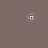
\includegraphics[width=0.4\linewidth]{images/red-maze-overlapping-step1.png}}%
    \caption{
        Resultat des ersten Zyklus mit dem Red-Maze Input. Da am Anfang die Entropie überall gleich ist, wird die Anfangszelle zufällig gewählt.
        Wenn der Algorithmus bereits die möglichen Module der benachbarten Zellen ausgewertet hat, dann werden die Zellen mit allen Farben der verwendbaren Modulen eingefärbt
        {(die Pixelfarben werden dann gemischt)}.
        Der direkt umliegende Bereich der Anfangszelle nicht in einer einheitlichen Farbe dargestellt, da es dort bereits weniger Optionen gibt die verwendet werden können \cite{Karth2017WaveFunctionCollapseIC}.
    }%
\end{figure}

\begin{figure}[H]
    \centering
    \frame{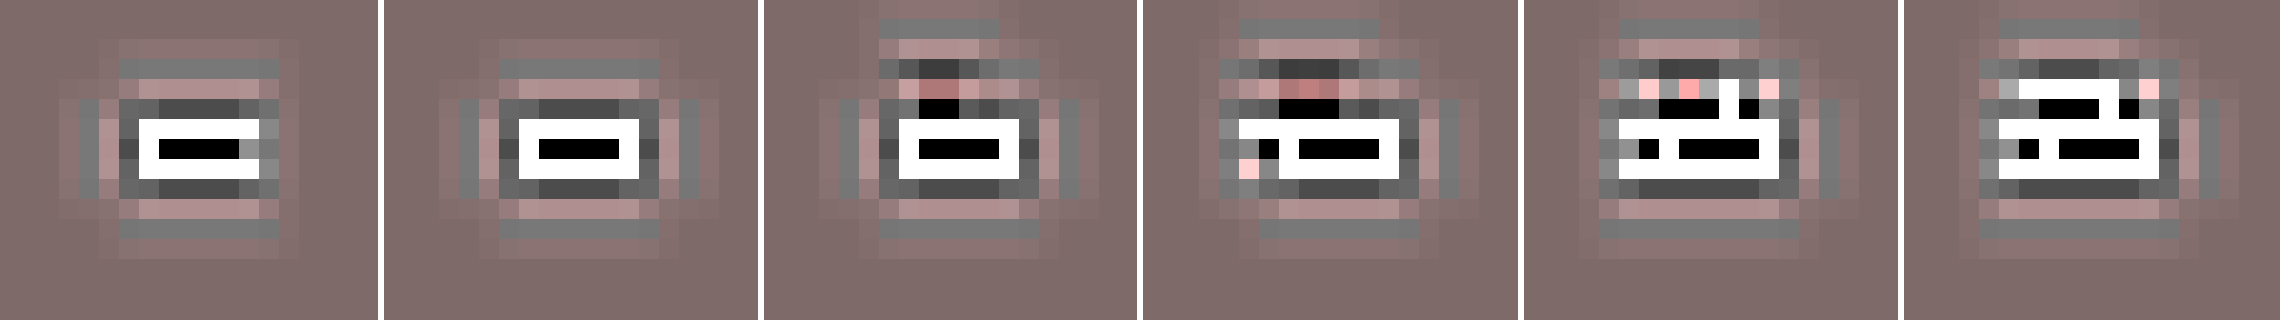
\includegraphics[width=1\linewidth]{images/red-maze-overlapping-steps.png}}%
    \caption{Die nächsten Zyklen für das Red-Maze Input \cite{Karth2017WaveFunctionCollapseIC}.}%
\end{figure}

\pagebreak

\section{Beispiel Implementierung}

In diesem Kapitel wird eine einfache Implementierung des WFC Algorithmus im Simple Tile Model, stellenweise als Pseudocode als auch als Programmcode, dargestellt.
Diese Implementierung wir dann um zwei Optimierungen erweitert.
Auf eine dieser Optimierungen wird mit Programmcode genauer erläutert, während die andere nicht implementiert, aber auf dessen Vorteile eingegangen wird.

\begin{lstlisting}
    init() {
        ladeModule();
        erstelleOutputZellen(); 
        fuelleOutputZellen();
        while(!alleZellenKollabiert) {
            sortiereZellenNachEntropie();
            kollabiereZelleMitNiedrigsterEntropy();
            for(jedeZelleImOutput) {
                berechneNachbarOptionen();
            }
            zeichneKollabierteZellen();
        }
    }
\end{lstlisting}

Zuerst werden die selbst erstellten Module geladen und in jeder einzelnen Zelle des Outputs werden alle Module hinzugefügt.
Dadruch erstellen wir ein CSP in der jede Zelle eine \textit{Superposition} besitzt.
In den Zeilen 5 bis 11 wird der Hauptteil von WFC ausgeführt.
Dort werden erst alle Zellen nach ihrer Entropie sortiert, sodass dann zufällig aus einer der niedrigsten Zellen ausgewählt werden kann.
Diese Zelle wir dann auf einen ihrer möglichen Eigenwerte kollabiert.
Damit haben wir den initialen \textit{Observation} Schritt.
Anschließend beginnt die \textit{Propagation}.
Hier wird durch jede nicht kollabierte Zelle Iteriert und die neuen möglichen Eigenwerte nach den bestimmten \textit{Constraints} errechnet.
Diese Zellen werden mit diesen neuen Eigenwerten aktualisiert.\par
\newpage
Um die Optimierung, die gleich vorgestellt wird, zu verdeutlichen wird auf die Funktion \texttt{ladeModule()} genauer eingegangen.

\begin{lstlisting}
    ladeModule() {
       modul[0]=new Tile(0,new Image(),[0,1,4],[0,1,2],[0,2,3],[0,3,4]);
       modul[1]=new Tile(1,new Image(),[2,3],[3,4],[0,2,3],[0,3,4]);
       modul[2]=new Tile(2,new Image(),[0,1,4],[3,4],[1,4],[0,3,4]);
       modul[3]=new Tile(3,new Image(),[0,1,4],[0,1,2],[1,4],[1,2]);
       modul[4]=new Tile(4,new Image(),[2,3],[0,1,2],[0,2,3],[1,2]);
       }
\end{lstlisting}

Die \texttt{ladeModule()} Funktion dient als Mapping der einzelnen Module.
Hier werden jedem Modul zusätzlich noch alle anderen Module, die an dieses Modul angrenzen können, festgelegt.
Die Reihenfolge der Optionen beginnt von Oben und rotiert im Uhrzeigersinn herum, damit alle vier Richtungen abgedeckt sind {(siehe Abbildung 3.17)}.
Das Problem an dieser Implementierung ist das mit Zunahme der Anzahl der Module auch die Komplexität und die Größe des Mappings zunimmt \cite{Shiffman}.

\begin{figure}[H]
    \centering
    \frame{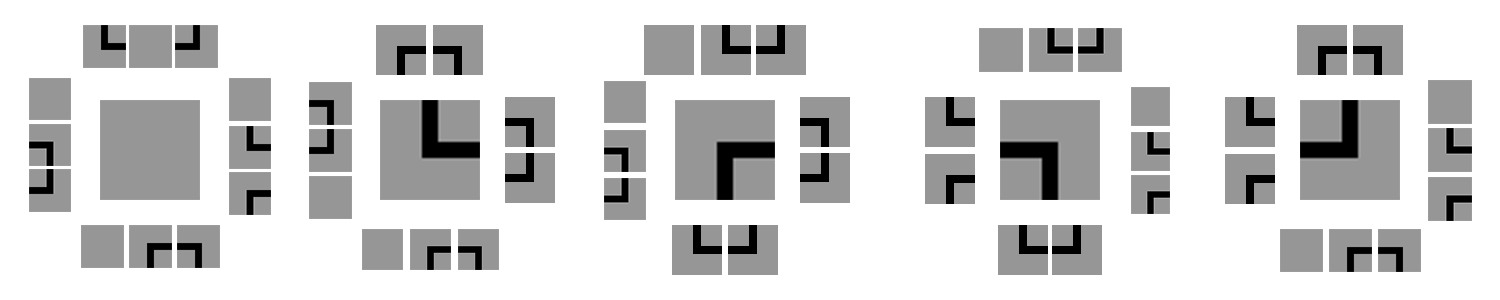
\includegraphics[width=1\linewidth]{images/simple-tile-mapping.png}}%
    \caption{Visualisierung eines Mappings der Module.}%
\end{figure}

Um das Mapping zu vereinfach können sogenannte \say{Sockets} verwendet werden.
Anstelle selbst zu entscheiden, welche Module an welche Module angeschlossen werden dürfen,
werden den Modulen an jeder Kante Sockets zugewiesen.
Dadurch können die Module selbst entscheiden welche Module an diese gesetzt werden dürfen,
indem die Sockets miteinander verglichen werden und nur Module mit identischen Sockets eine gültige Verbindung sind \cite{Shiffman}.

\begin{lstlisting}
    ladeModule() {
       modul[0]= new Tile(0,'/maze/0.png','AAA','AAA','AAA','AAA');
       modul[1]= new Tile(1,'/maze/1.png','ABA','ABA','AAA','AAA');
       modul[2]= new Tile(2,'/maze/2.png','AAA','ABA','ABA','AAA');
       modul[3]= new Tile(3,'/maze/3.png','AAA','AAA','ABA','ABA');
       modul[4]= new Tile(4,'/maze/4.png','ABA','AAA','AAA','ABA');
       }
\end{lstlisting}

Die Sockets werden hier ebenfalls beginnend von Oben und rotierend im Uhrzeigersinn zugewiesen.
Es muss darauf geachtet werden das die Sockets konsistent für alle Module nach demselben Prinzip zugewiesen werden.
In diesem fall werden sie strikt um Uhrzeigersinn ungeachtet der natürlichen Schreibrichtung zugewiesen {(siehe Abbildung 3.18)}.
Durch die Verwendung von Sockets lässt sich die Komplexität und somit die Erstellung des Mappings stark reduzieren \cite{Shiffman}.

\begin{figure}[H]
    \centering
    \frame{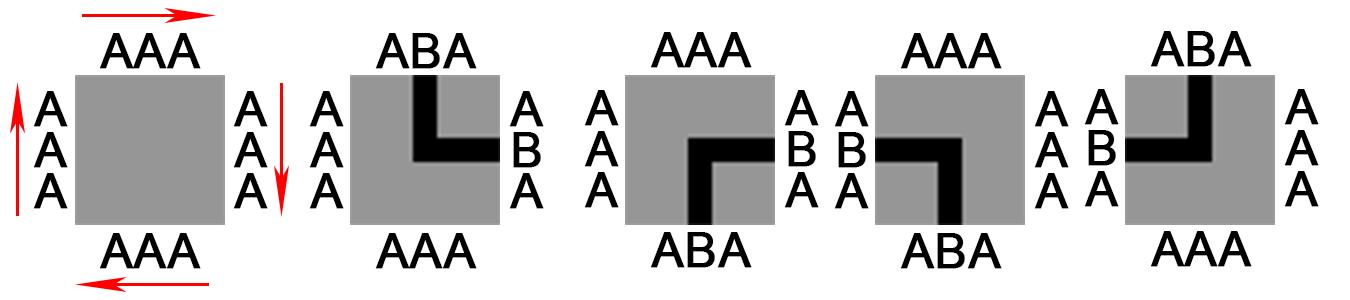
\includegraphics[width=1\linewidth]{images/simple-tile-sockets.png}}%
    \caption{Visualisierung eines Mappings mit Sockets.}%
\end{figure}

Wenn Sockets verwendet werden, dann müssen auch dazu passende Module verwendet werden.
Werden einfarbige Module verwendet, wie z.B. Module für Wald, Wiese, Strand und Meer,
dann können die Sockets das Mapping verkomplizieren anstatt zu vereinfachen.
In diesen Fällen benötigen die Module Verbindungsmodule und Eckmodule, um alle nötigen Kombinationen zu ermöglichen {(siehe Abbildung 3.8 (a))}.
Dadurch verändert sich der Output dahingehen, das \say{halbe} Terrains zustande kommen.

Eine weitere Optimierung vorgeschlagen von Boris ist, das nur die Zellen auf Constaints geprüft werden,
die durch den Propagation Vorgang zu anderen Ergebnissen führen können.
Das bedeutet, wenn eine Zelle aktualisiert wird, dann fügen wir sie einer Warteschlange ausstehender Zellen hinzu.
Dann werden die ausstehenden Zellen einer nach der anderen aus der Warteschlange entfernt und auf ihren Nachbarzellen geprüft.
Sollten die Nachbarzellen dazu führen, dass weitere Zellen aktualisiert werden müssen, dann werden diese ebenfalls zu Warteschlange hinzugefügt.
Dieser Vorgang wird so lange wiederholt bis die Warteschlange leer ist.
Dadruch haben wir sichergestellt,
dass jeder Constraint vollständig ausgewertet wurde, aber wir überprüfen nie ein Constraint,
es sei denn, eine der mit ihr verbundenen Zellen hat ihren Eigenwert geändert.
Diese Optimierung erhöht die Geschwindigkeit von WFC maßgeblich \cite{boris}.

\pagebreak
\subsection{Weitere Implementierungen von WFC}

Joseph Parker war einer der ersten Entwickler, der WFC verwendet hat.
In seinem in der Unity Engine entwickeltem Spiel \textit{Proc Skater 2016} verwendet er den Algorithmus, um einzigartige 3D Skateparks zu generieren.
In Abbildung 3.19 dargestellt seine selbst erstellten Blöcke, aus denen die Karte generiert werden soll {(Abbildung 3.20)}, anstatt sie automatisch aus einem Input zu analysieren \cite{procskater2016}.
J. Parker zufolge benutzt er das Simple Tile Model, als auch das Overlapping Model für den Skatepark. \footnote[5]{Persönliche Kommunikation, 23. Mai 2023}

\begin{figure}[H]
    \centering
    \includegraphics[width=0.9\linewidth]{images/proc-skater-ruleset.png}%
    \caption{Blöcke zu Generierung des Skateparks in \textit{Proc Skater 2016} \cite{procskater2016}.}%
\end{figure}

Die adjacency constraints für diese Blöcke werden aus einer ruleset $.xml$ ausgelesen und angewendet.

\begin{figure}[H]
    \centering
    \includegraphics[width=0.9\linewidth]{images/proc-skate-level.png}%
    \caption{Typisches Level in \textit{Proc Skater 2016} \cite{procskater2016}.}%
\end{figure}


\begin{wrapfigure}{r}{8cm}
    \includegraphics[width=1\linewidth]{images/proc-skate-backdrop.png}%
    \caption{Overlapping Model für das Backdrop in \textit{Proc Skater 2016} \cite{procskater2016}.}%
\end{wrapfigure}

Das Overlapping Model verwendete er um den umliegenden Hintergrund \textit{(backdrop)} für seinen Skatepark in Abbildung 3.21 zu erstellen.
Weiter erklärte Parker, dass das Tile Model und das Overlapping Model sich jeweils für unterschiedliche Bereiche gut anwenden lassen.
\say{Das Tile Model ist besser für Straßen, Labyrinthe oder alles mit formalen Übergängen.
Overlapping Model für Plattform artige Situationen, in denen man eher eine Art Markow-Kette für die Größe der Features haben möchte.}
\footnote[5]{Persönliche Kommunikation, 23. Mai 2023}
\newline
Eine weitere kommerzielle Implementierung von WFC ist \textit{Caves of Qud}, entwickelt von Freehold Games.
Laut Brian Bucklew, einem der Entwickler bei Freehold Games, verwendet \textit{Caves of Qud} einen Mehrfachdurchlauf \textit{(multipass)} von WFC.
Dadurch können größere Komplexitäten bei der Generierung von Karten erreicht werden wie in Abbildung 3.22.
Ein weiterer Vorteil, der sich durch WFC ergeben hat, ist die einfache Handhabung.
Sobald das zugrunde liegende System vorhanden ist, kann jeder Entwickler Input-Images einspielen und spielbaren Content generieren.
\footnote[6]{Aus Forums-Korrespondenz \url{https://forums.somethingawful.com/showthread.php?threadid=3563643&userid=68893&perpage=40&pagenumber=23\#post467126402}} \cite{Karth2017WaveFunctionCollapseIC}

\begin{figure}[H]
    \centering
    \frame{\includegraphics[width=0.9\linewidth]{images/caves-of-qud.jpg}}%
    \caption{Zwei Spielbare Karten von \textit{Caves of Qud} \cite{Karth2017WaveFunctionCollapseIC}.}%
\end{figure}

Wave-Function-Collapse kann nicht nur auf flachen Ebenen mit quadratischen Zellen verwenden werden \cite{boris}.
Oskar Stålberg verwendete WFC nicht nur im 2D und 3D-Raum, sondern auch auf irregulären Rastern.
In einem Beispiel implementiert Stålberg WFC auf einer Sphäre mit einem Dreiecks-Raster.
\footnote[7]{Beispiele auf seiner Website
\url{https://oskarstalberg.tumblr.com/}
oder seinem Twitter
\url{https://twitter.com/OskSta/status/784847588893814785}}

\chapter{Fazit}

Der Wave-Function-Collapse Algorithmus von Gumin sowie die Model Synthese von Paul Merrell haben mehr Gemeinsamkeiten als Unterschiede.
Das liegt daran, dass beide Algorithmen denselben grundlegenden Ablauf für das Lösen von Constraint-Satisfaction-Problem verwenden.
Beide Algorithmen kann man als jeweils eine Seite derselben Münze bezeichnen.
Wave-Function-Collapse ist essenziell ein Verfahren um einzelne Elemente, ob Blöcke, Texte, Bilder etc. nach bestimmten Regeln aneinander zu setzten.
Dadurch lassen sich mit beiden Algorithmen fehlerfreie Systeme, die gegebenenfalls Interaktiv verwendet werden können, automatisch generieren.
Die Unterschiede zwischen den beiden Algorithmen sind hauptsächlich in der Implementierung der einzelnen Ausführungsschritte sowie in zusätzlichen Optimierungen zu finden.
Der WFC von Gumin verwendet das Overlapping Model, um die Generierung der Bausteine / Module zu vereinfachen.
Die dadurch dichtere Platzierung der einzelnen Zellen führt zu einem einheitlicherem Output, kann aber zur Folge haben das Artefakte entstehen,
sollte die Fenstergröße für die Analyse nicht korrekt gewählt worden sein.
Die Model Synthese von Paul Merrell hingegen besitzt Fehlerbehandlungen wie die blockweise Generierung bei der Ausführung des Algorithmus, um größere Outputs zu erzielen und die
Fehlerrate zu reduzieren.
Beide Implementierungen können um weitere Funktionalitäten erweitert werden, um dieselben oder mehr Funktionalitäten zu erhalten.

\printbibliography

\chapter{Anhang}

\begin{figure}[H]
    \centering
    \includegraphics[width=0.45\linewidth]{images/wfc-model-comparison/summer-modelsynthesis.png}%
    \qquad
    \includegraphics[width=0.45\linewidth]{images/wfc-model-comparison/summer-wfc.png}%
    \vspace{1em}
    \includegraphics[width=0.45\linewidth]{images/wfc-model-comparison/castle-model.png}%
    \qquad
    \includegraphics[width=0.45\linewidth]{images/wfc-model-comparison/kein-resultat.png}%
    \caption{Texturen Links mit Model Synthese generiert. Texturen Rechts mit WFC. \cite[S.10]{merrell2018compare}.}%
\end{figure}

\begin{figure}[H]
    \centering
    \includegraphics[width=0.45\linewidth]{images/wfc-model-comparison/knot-1-model.png}%
    \qquad
    \includegraphics[width=0.45\linewidth]{images/wfc-model-comparison/knot-1-wfc.png}%
    \vspace{1em}
    \includegraphics[width=0.45\linewidth]{images/wfc-model-comparison/knot-2-model.png}%
    \qquad
    \includegraphics[width=0.45\linewidth]{images/wfc-model-comparison/kein-resultat.png}%
    \caption{Texturen Links mit Model Synthese generiert. Texturen Rechts mit WFC. \cite[S.11]{merrell2018compare}.}%
\end{figure}

\begin{figure}[H]
    \centering
    \includegraphics[width=0.45\linewidth]{images/wfc-model-comparison/knot-3-model.png}%
    \qquad
    \includegraphics[width=0.45\linewidth]{images/wfc-model-comparison/knot-3-wfc.png}%
    \vspace{1em}
    \includegraphics[width=0.45\linewidth]{images/wfc-model-comparison/knot-4-model.png}%
    \qquad
    \includegraphics[width=0.45\linewidth]{images/wfc-model-comparison/knot-4-wfc.png}%
    \caption{Texturen Links mit Model Synthese generiert. Texturen Rechts mit WFC. \cite[S.12]{merrell2018compare}.}%
\end{figure}

\begin{figure}[H]
    \centering
    \includegraphics[width=0.45\linewidth]{images/wfc-model-comparison/red-dot-model.png}%
    \qquad
    \includegraphics[width=0.45\linewidth]{images/wfc-model-comparison/kein-resultat.png}%
    \vspace{1em}
    \includegraphics[width=0.45\linewidth]{images/wfc-model-comparison/shrew-model.png}%
    \qquad
    \includegraphics[width=0.45\linewidth]{images/wfc-model-comparison/kein-resultat.png}%
    \vspace{1em}
    \includegraphics[width=0.45\linewidth]{images/wfc-model-comparison/cat-model.png}%
    \qquad
    \includegraphics[width=0.45\linewidth]{images/wfc-model-comparison/kein-resultat.png}%
    \caption{Texturen Links mit Model Synthese generiert. Texturen Rechts mit WFC. \cite[S.13]{merrell2018compare}.}%
\end{figure}

\end{document}